% =============================================================
%  MechanicPro --- User Manual
%  Template: Professional / Modern / Clean
% =============================================================

\documentclass[12pt, a4paper]{report}

% -- Encoding & Font ------------------------------------------
\usepackage[T1]{fontenc}
\usepackage[utf8]{inputenc}
\usepackage[scaled=0.92]{helvet}
\renewcommand{\familydefault}{\sfdefault}

% -- Page Layout ----------------------------------------------
\usepackage[
top=2.5cm, bottom=2.5cm,
left=3cm,  right=2.5cm
]{geometry}
% Automatic "Month Year" date
\newcommand{\monthyear}{%
	\ifcase\month\or January\or February\or March\or April\or May\or June\or
	July\or August\or September\or October\or November\or December\fi
	\space\the\year%
}
\usepackage{parskip}
\usepackage{float}

% -- Colors ---------------------------------------------------
\usepackage{xcolor}
\definecolor{Navy}{RGB}{15, 40, 75}
\definecolor{Blue}{RGB}{37, 99, 195}
\definecolor{LightBlue}{RGB}{219, 234, 254}
\definecolor{TextGray}{RGB}{90, 105, 120}
\definecolor{LightGray}{RGB}{248, 249, 251}
\definecolor{RuleGray}{RGB}{220, 225, 232}
\definecolor{StatusGreen}{RGB}{22, 163, 74}
\definecolor{WarnYellow}{RGB}{254, 243, 199}
\definecolor{WarnBorder}{RGB}{217, 119, 6}
\definecolor{DangerRed}{RGB}{254, 226, 226}
\definecolor{DangerBorder}{RGB}{185, 28, 28}

% -- Graphics & Drawing ---------------------------------------
\usepackage{graphicx}
\usepackage{tikz}
\usetikzlibrary{calc}

% -- Tables ---------------------------------------------------
\usepackage{booktabs}
\usepackage{tabularx}
\usepackage{array}
\usepackage{longtable}

% -- Lists ----------------------------------------------------
\usepackage{enumitem}
\setlist[itemize]{leftmargin=1.5em, itemsep=3pt}
\setlist[enumerate]{leftmargin=1.5em, itemsep=3pt}

% Compact step list (numbered, used for procedures)
\newlist{steps}{enumerate}{1}
\setlist[steps]{
	label=\textbf{\color{Blue}\arabic*.},
	leftmargin=2em,
	itemsep=5pt,
	topsep=6pt,
}

% -- Headers & Footers ----------------------------------------
\usepackage{fancyhdr}
\pagestyle{fancy}
\fancyhf{}
\fancyhead[L]{%
	\small\color{TextGray}\textit{MechanicPro \textemdash{} User Manual}%
}
\fancyhead[R]{%
	\small\color{TextGray}v1.0.0%
}
\fancyfoot[L]{%
	\small\color{TextGray}User Manual%
}
\fancyfoot[R]{%
	\small\color{TextGray}\thepage%
}
\renewcommand{\headrulewidth}{0.4pt}
\renewcommand{\footrulewidth}{0.4pt}
\renewcommand{\headrule}{%
	\color{RuleGray}\hrule width\headwidth height\headrulewidth%
}
\renewcommand{\footrule}{%
	\color{RuleGray}\hrule width\headwidth height\footrulewidth%
}

% Plain style for chapter-opening pages
\fancypagestyle{plain}{%
	\fancyhf{}
	\fancyfoot[R]{\small\color{TextGray}\thepage}
	\renewcommand{\headrulewidth}{0pt}
	\renewcommand{\footrulewidth}{0.4pt}
	\renewcommand{\footrule}{%
		\color{RuleGray}\hrule width\headwidth height\footrulewidth%
	}
}

% -- Section Formatting ---------------------------------------
\usepackage{titlesec}

\titleformat{\chapter}[block]
{\normalfont\huge\bfseries\color{Navy}}
{\color{Blue}\thechapter}{1em}{}
[\vspace{4pt}\color{Blue}\rule{\textwidth}{1.5pt}\vspace{-6pt}]

\titlespacing{\chapter}{0pt}{0pt}{20pt}

\titleformat{\section}
{\normalfont\Large\bfseries\color{Navy}}
{\color{Blue}\thesection}{1em}{}

\titleformat{\subsection}
{\normalfont\large\bfseries\color{TextGray}}
{\thesubsection}{1em}{}

\titleformat{\subsubsection}
{\normalfont\normalsize\bfseries\color{TextGray}}
{\thesubsubsection}{1em}{}

% -- TOC Styling ----------------------------------------------
\usepackage{tocloft}
\renewcommand{\cftchapfont}{\bfseries\color{Navy}}
\renewcommand{\cftchappagefont}{\bfseries\color{Navy}}
\renewcommand{\cftsecfont}{\color{TextGray}}
\renewcommand{\cftsecpagefont}{\color{TextGray}}
\setlength{\cftbeforechapskip}{6pt}

% -- Hyperlinks -----------------------------------------------
\usepackage{hyperref}
\hypersetup{
	colorlinks  = true,
	linkcolor   = Blue,
	urlcolor    = Blue,
	citecolor   = Blue,
	pdftitle    = {MechanicPro - User Manual},
	pdfauthor   = {Eduardo Freitas Fernandes},
	pdfsubject  = {User Manual},
	pdfkeywords = {MechanicPro, mechanic shop, user manual},
}

% -- Custom Commands ------------------------------------------

% Note box (blue)
\newcommand{\notebox}[1]{%
	\vspace{6pt}
	\noindent
	\colorbox{LightBlue}{%
		\begin{minipage}{\dimexpr\linewidth-2\fboxsep}%
			\vspace{5pt}
			\small\textbf{\color{Blue}Note:\space}\color{Navy}#1
			\vspace{5pt}
		\end{minipage}%
	}
	\vspace{6pt}
}

% Warning box (yellow)
\newcommand{\warnbox}[1]{%
	\vspace{6pt}
	\noindent
	\colorbox{WarnYellow}{%
		\begin{minipage}{\dimexpr\linewidth-2\fboxsep}%
			\vspace{5pt}
			\small\textbf{\color{WarnBorder}Warning:\space}\color{Navy}#1
			\vspace{5pt}
		\end{minipage}%
	}
	\vspace{6pt}
}

% Danger box (red) -- for destructive actions
\newcommand{\dangerbox}[1]{%
	\vspace{6pt}
	\noindent
	\colorbox{DangerRed}{%
		\begin{minipage}{\dimexpr\linewidth-2\fboxsep}%
			\vspace{5pt}
			\small\textbf{\color{DangerBorder}Caution:\space}\color{Navy}#1
			\vspace{5pt}
		\end{minipage}%
	}
	\vspace{6pt}
}

% UI element label (buttons, menus, field names)
\newcommand{\ui}[1]{\textbf{\color{Navy}#1}}

% Keyboard shortcut
\newcommand{\key}[1]{%
	\tikz[baseline=(k.base)]\node[
	draw=RuleGray, fill=LightGray, rounded corners=2pt,
	inner xsep=4pt, inner ysep=2pt, font=\small\ttfamily
	](k){#1};%
}

% -- Abstract Page --------------------------------------------
\newcommand{\abstractpage}[1]{%
	\clearpage
	\thispagestyle{plain}
	\vspace*{2cm}
	\begin{center}
		{\color{Navy}\Large\bfseries Abstract}\\[0.4cm]
		\color{Blue}\rule{0.3\textwidth}{1.5pt}
	\end{center}
	\vspace{0.8cm}
	\begin{quote}
		\setlength{\parskip}{6pt}
		\normalsize #1
	\end{quote}
	\vfill
	\noindent\small\color{TextGray}
	\textbf{Keywords:} MechanicPro, user manual, mechanic shop,
	service orders, clients, vehicles, CSV, PDF.
	\clearpage
}

% -- Cover Page -----------------------------------------------
\newcommand{\coverpage}{%
	\begin{titlepage}
		\begin{tikzpicture}[remember picture, overlay]
			
			%% Top bar
			\fill[Navy]
			(current page.north west)
			rectangle
			([yshift=-4cm] current page.north east);
			
			%% Accent stripe
			\fill[Blue]
			([yshift=-4cm] current page.north west)
			rectangle
			([yshift=-4.12cm] current page.north east);
			
			%% Bottom band
			\fill[LightGray]
			(current page.south west)
			rectangle
			([yshift=3.2cm] current page.south east);
			
			%% Bottom band top border
			\fill[RuleGray]
			([yshift=3.2cm] current page.south west)
			rectangle
			([yshift=3.24cm] current page.south east);
			
		\end{tikzpicture}
		
		%% -- Top bar content -----------------------
		\vspace*{1.2cm}
		\hspace{1.2cm}
		\begin{minipage}{0.8\textwidth}
			{\color{white}\footnotesize\bfseries\MakeUppercase{User Manual}}
			\quad
			{\color{Blue!40!white}\footnotesize User Manual}
		\end{minipage}
		
		\vspace{3.6cm}
		
		%% -- Main title block ----------------------
		\hspace{1.2cm}
		\begin{minipage}{0.82\textwidth}
			
			{\color{Navy}\Huge\bfseries\scalebox{2.0}{MechanicPro}}
			
			\vspace{0.3cm}
			{\color{TextGray}\large Management System for a Mechanic Shop}
			
			\vspace{0.6cm}
			\color{Blue}\rule{\textwidth}{1.5pt}
			\vspace{0.3cm}
			
			{\color{TextGray}\normalsize
				Complete Guide to Installation, Daily Use, and Data Management
			}
			
		\end{minipage}
		
		\vfill
		
		%% -- Metadata block ------------------------
		\hspace{1.2cm}
		\begin{minipage}{0.82\textwidth}
			\renewcommand{\arraystretch}{1.5}
			\begin{tabular}{>{\color{TextGray}\small\bfseries}l
					>{\small}l
					@{\hskip 2cm}
					>{\color{TextGray}\small\bfseries}l
					>{\small}l}
				Author    & Eduardo Freitas Fernandes      & Version   & 1.0.0      \\
				Date      & \monthyear     & Status    &
				\textcolor{StatusGreen}{\bfseries Final}        \\
				Document  & User Manual & Language  & English    \\
			\end{tabular}
		\end{minipage}
		
		\vspace{2.8cm}
		
	\end{titlepage}
}

% =============================================================
%  DOCUMENT
% =============================================================

\begin{document}
	
	\coverpage
	
	\abstractpage{%
		This document is the user manual for \textbf{MechanicPro}, a desktop
		application for managing the operations of a mechanic shop. It covers
		everything a user needs to install and run the application, navigate its
		interface, and perform all available tasks.
		
		The manual is organised by workflow. Each chapter corresponds to a
		distinct area of the application: managing clients and vehicles, handling
		service orders, using the dashboard, and working with data import,
		export, and PDF generation.
		
		No technical knowledge is required to follow this manual. For information
		about the system architecture or database design, refer to the Technical
		Report (TR-MECHPRO-001).
	}
	
	% -- Revision History -----------------------------------------
	\chapter*{Revision History}

	This section outlines the revision history of the document.

	\begin{table}[H]
		\centering
		\begin{tabularx}{\textwidth}{c l X l}
			\toprule
			\textbf{Version} & \textbf{Date} & \textbf{Description} & \textbf{Author} \\
			\midrule
			1.0.0 & June 2026 & Initial document created           & Eduardo Freitas Fernandes \\
			\bottomrule
		\end{tabularx}
	\end{table}
	
	\newpage
	
	\tableofcontents
	
	\newpage
	
	\listoffigures
	
	\newpage
	
	\listoftables
	
	
	% =============================================================
	%  CHAPTER 1 --- INTRODUCTION
	% =============================================================
	\chapter{Introduction}
	
	\section{About This Manual}
	This manual is designed to guide you through the installation, setup, and daily use of MechanicPro. It provides step-by-step instructions for managing your shop's core operations, including clients, vehicles, and service orders.
	
	The document is structured sequentially, starting from basic installation and interface navigation, progressing to core workflows like creating service orders, and finishing with data management tasks such as CSV exports and PDF generation. 
	
	This manual is intended for end-users: shop owners, managers, and mechanics. It covers the practical application of the software. It does \emph{not} cover technical architecture, database design, or developer setup.
	
	\section{About MechanicPro}
	MechanicPro is a fast, secure, and easy-to-use desktop application specifically designed for mechanic shops. It replaces paper records and complicated spreadsheets with a streamlined digital system.
	
	With MechanicPro, you can:
	\begin{itemize}
		\item Register clients and their vehicles.
		\item Track service orders, including parts, labor, and mileage.
		\item Monitor your shop's performance via an interactive dashboard.
		\item Print or download professional PDF invoices for your customers.
		\item Back up your data at any time via CSV export.
	\end{itemize}
	
	\notebox{MechanicPro runs entirely offline. All your data is stored securely on your local computer, ensuring complete privacy and fast access without requiring an internet connection.}
	
	\section{Conventions Used in This Manual}
	
	Throughout this document the following conventions are used:
	
	\begin{itemize}
		\item \ui{Bold navy text} refers to interface elements such as buttons,
		menu items, and field labels.
		\item \key{Ctrl+S} represents keyboard shortcuts.
		\item Steps to complete a task are numbered and shown like this:
	\end{itemize}
	
	\begin{steps}
		\item This is how a step looks.
		\item Each step describes one action.
	\end{steps}
	
	\notebox{Blue boxes contain tips or additional context.}
	
	\warnbox{Yellow boxes highlight situations that may produce unexpected results.}
	
	\dangerbox{Red boxes warn about irreversible actions, such as deleting records.}
	
	% =============================================================
	%  CHAPTER 2 --- INSTALLATION
	% =============================================================
	\chapter{Installation}
	
	\section{System Requirements}
	
	The hardware and software requirements to run the application are listed in Table~\ref{tab:system_requirements}.
	
	\begin{table}[H]
		\centering
		\caption{System Requirements}
		\label{tab:system_requirements}
		\begin{tabularx}{\textwidth}{l X}
			\toprule
			\textbf{Component} & \textbf{Requirement} \\
			\midrule
			Operating System & Windows 10 or later / macOS 11 or later / Ubuntu 20.04 or later \\
			RAM              & 4 GB minimum, 8 GB recommended \\
			Disk Space       & 50 MB minimum (additional space required for database growth) \\
			Additional       & Windows: WebView2 runtime (included in Windows 11) \\
			\bottomrule
		\end{tabularx}
	\end{table}
	
	\section{Installing the Application}
	
	\subsection{Windows}
	
	\begin{steps}
		\item Download the \texttt{MechanicPro\_1.0.0\_x64.msi} installer.
		\item Double-click the installer file.
		\item Follow the on-screen instructions.
		\item Launch \ui{MechanicPro} from the Start Menu or the desktop shortcut.
	\end{steps}
	
	\notebox{Windows may show a security warning on first launch because the
		application is not signed with a commercial certificate. Click
		\ui{More info} and then \ui{Run anyway} to proceed.}
	
	\subsection{macOS}
	
	\begin{steps}
		\item Download the \texttt{MechanicPro\_1.0.0\_x64.dmg} file.
		\item Open the \texttt{.dmg} and drag \ui{MechanicPro} to your
		\ui{Applications} folder.
		\item On first launch, right-click the app and select \ui{Open}.
	\end{steps}
	
	\subsection{Linux}
	
	\begin{steps}
		\item Download the \texttt{.deb} or \texttt{.AppImage} package.
		\item Install with \texttt{sudo dpkg -i MechanicPro\_1.0.0\_amd64.deb}
		or make the AppImage executable and run it directly.
	\end{steps}
	
	\section{First Launch}
	When you open MechanicPro for the very first time, the application will automatically set up your secure, local database file. This process is instant and requires no configuration on your part.
	
	Because the database is new, your \ui{Dashboard} will be empty, showing zero clients, vehicles, and service orders. You are now ready to begin adding your shop's data.
	
	\notebox{MechanicPro stores all data locally on your machine. No account or
		internet connection is required.}
	
	% =============================================================
	%  CHAPTER 3 --- INTERFACE OVERVIEW
	% =============================================================
	\chapter{Interface Overview}
	
	\section{Main Window}
	The MechanicPro window is divided into two primary areas: the \textbf{Sidebar} on the left, which contains the main navigation menu, and the \textbf{Main Content Area} on the right, which displays the currently selected view (see Figure~\ref{fig:main_content}).
	
    \begin{figure}[H]
		\centering
		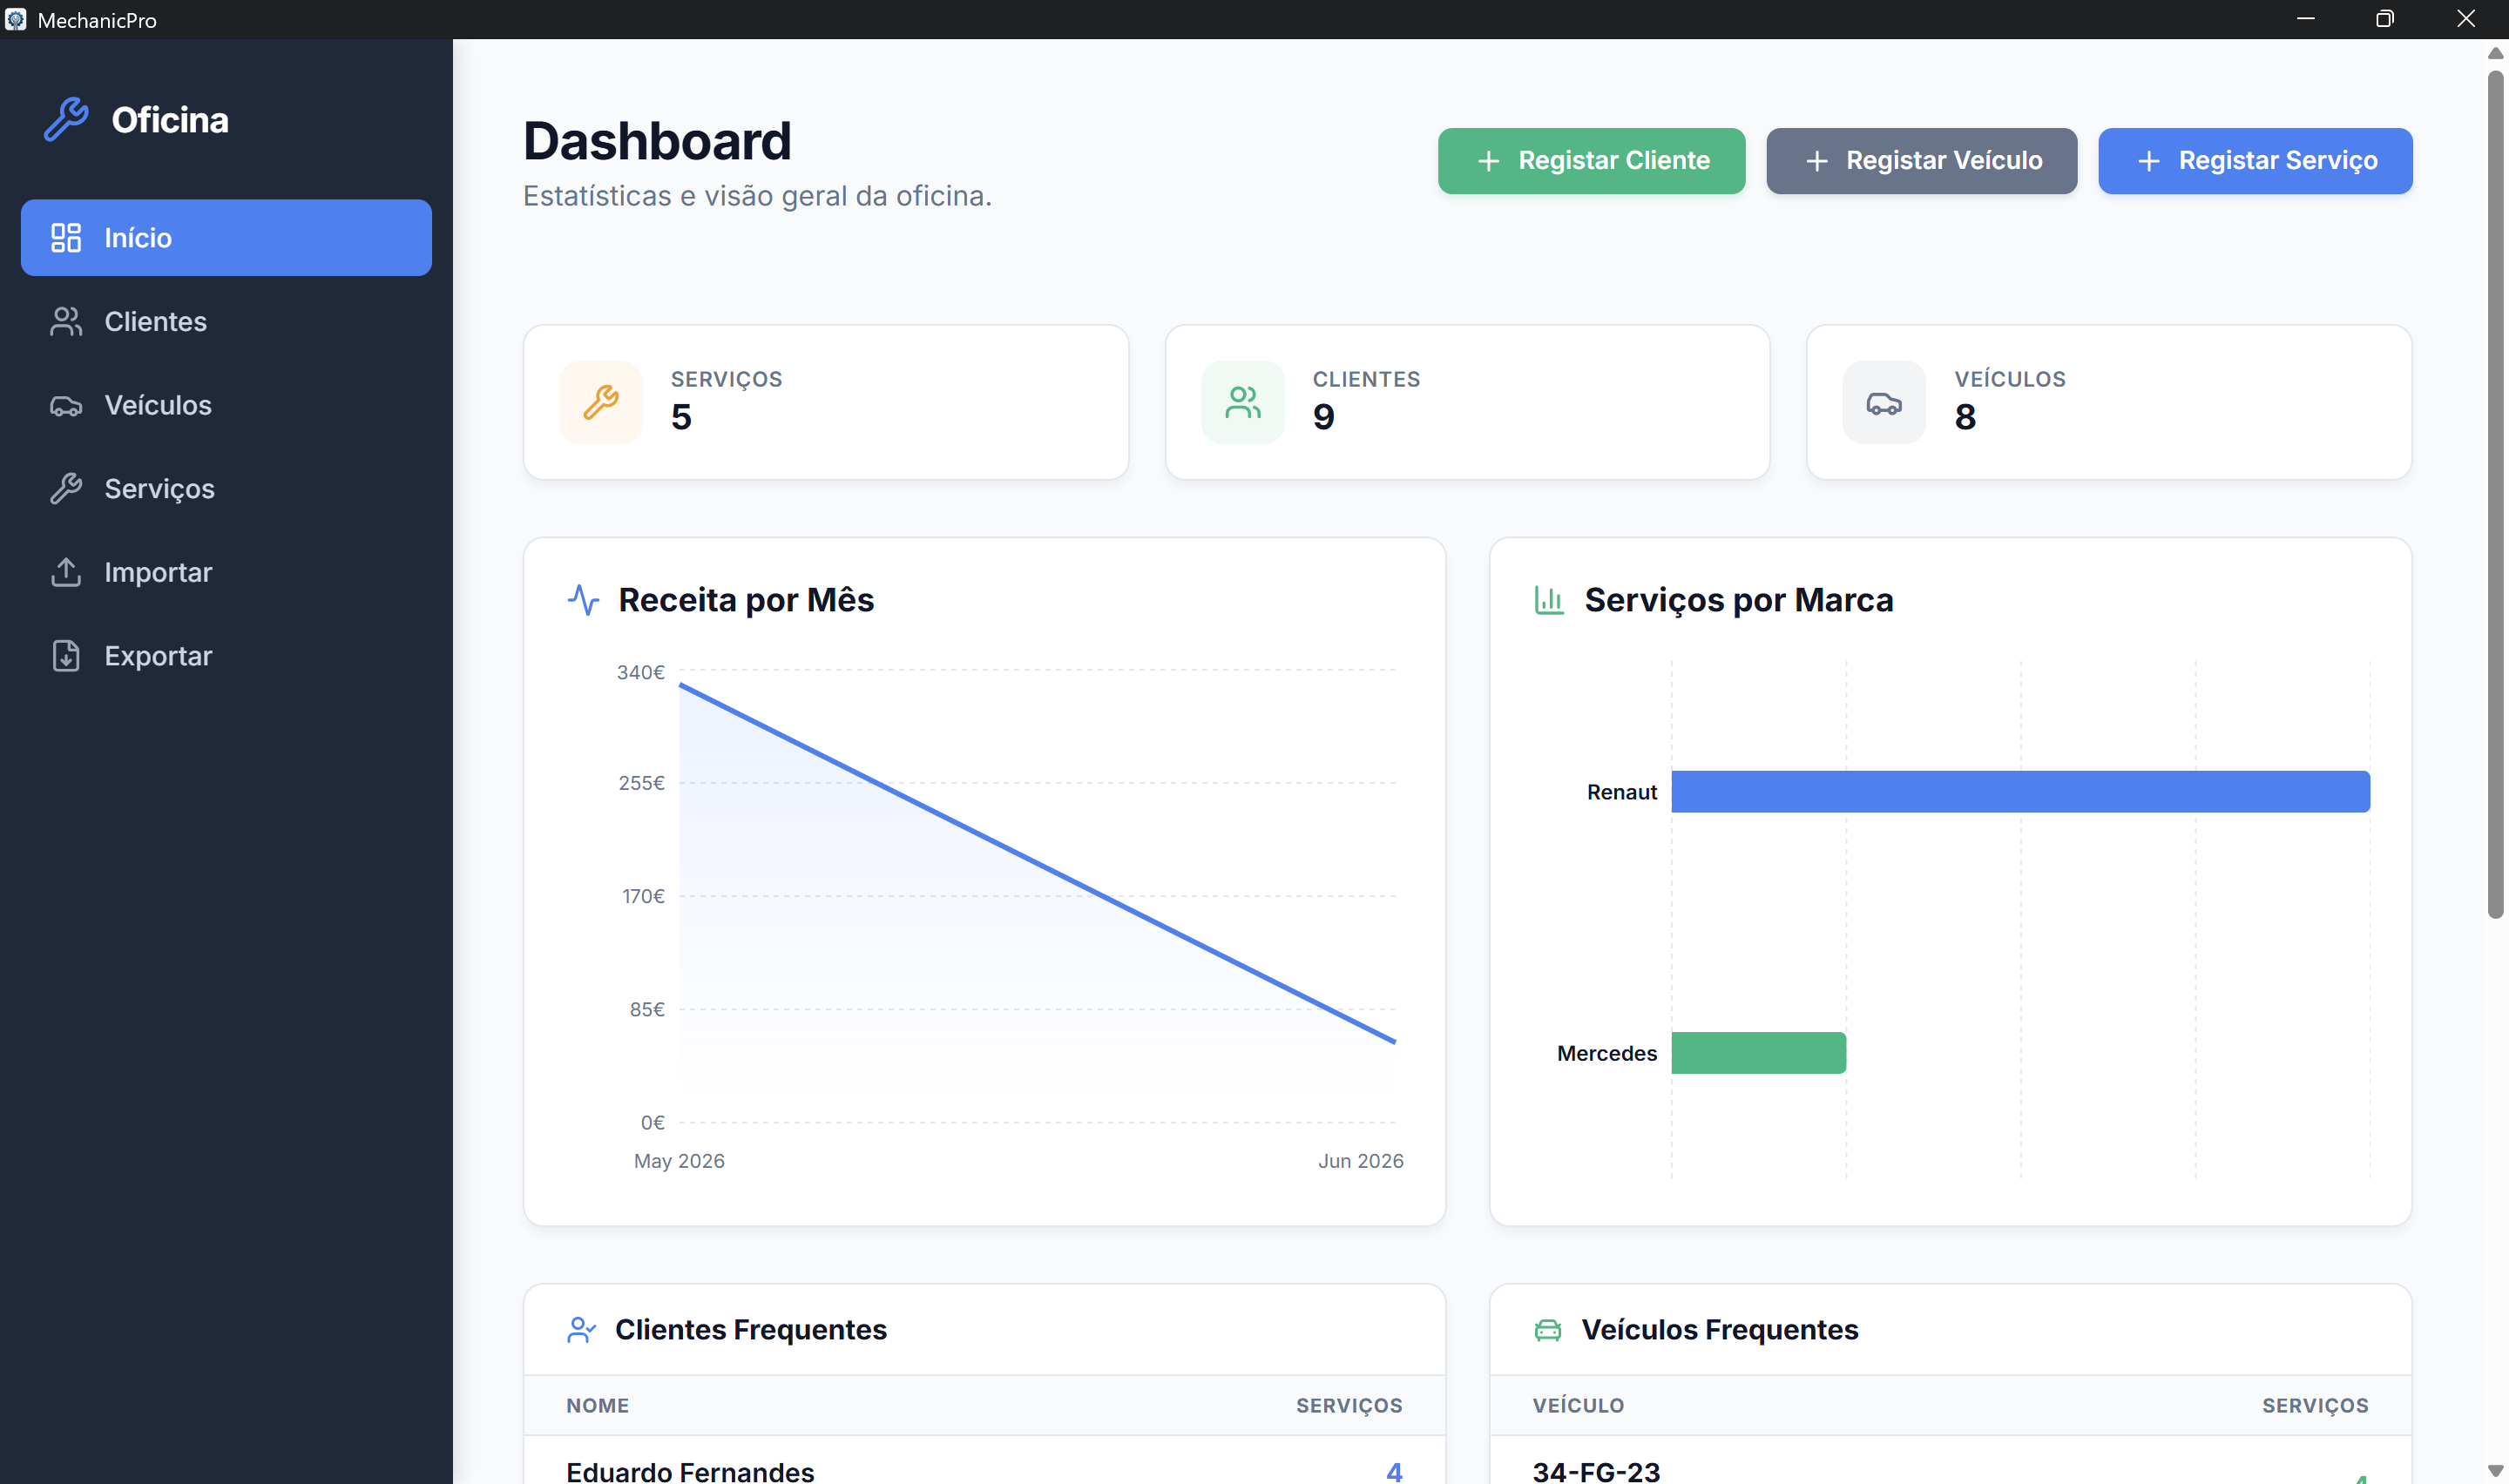
\includegraphics[width=0.9\textwidth]{figures/sidebar_main_content.png}
		\caption{Main Page}
		\label{fig:main_content}
	\end{figure}
	
	\section{Navigation}
	You can move between different sections of the application using the links in the left sidebar. Your current search filters and sorting preferences are remembered as you navigate between pages.
	
	The main sections are:
	\begin{itemize}
		\item \ui{Dashboard}: Summary statistics and shop performance charts.
		\item \ui{Clients}: Manage the vehicle owners in your system.
		\item \ui{Vehicles}: Manage the cars registered to your clients.
		\item \ui{Service Orders}: Create, edit, and track repair and maintenance jobs.
		\item \ui{Import / Export}: Backup and migrate your data using CSV files.
	\end{itemize}
	
	\section{Dashboard}
	When you launch the application, you will land on the Dashboard. This screen provides a high-level overview of your shop's operations, showing the total number of clients, active vehicles, and the status of recent service orders (see Figure~\ref{fig:dashboard_page}).
	
	\begin{figure}[H]
		\centering
		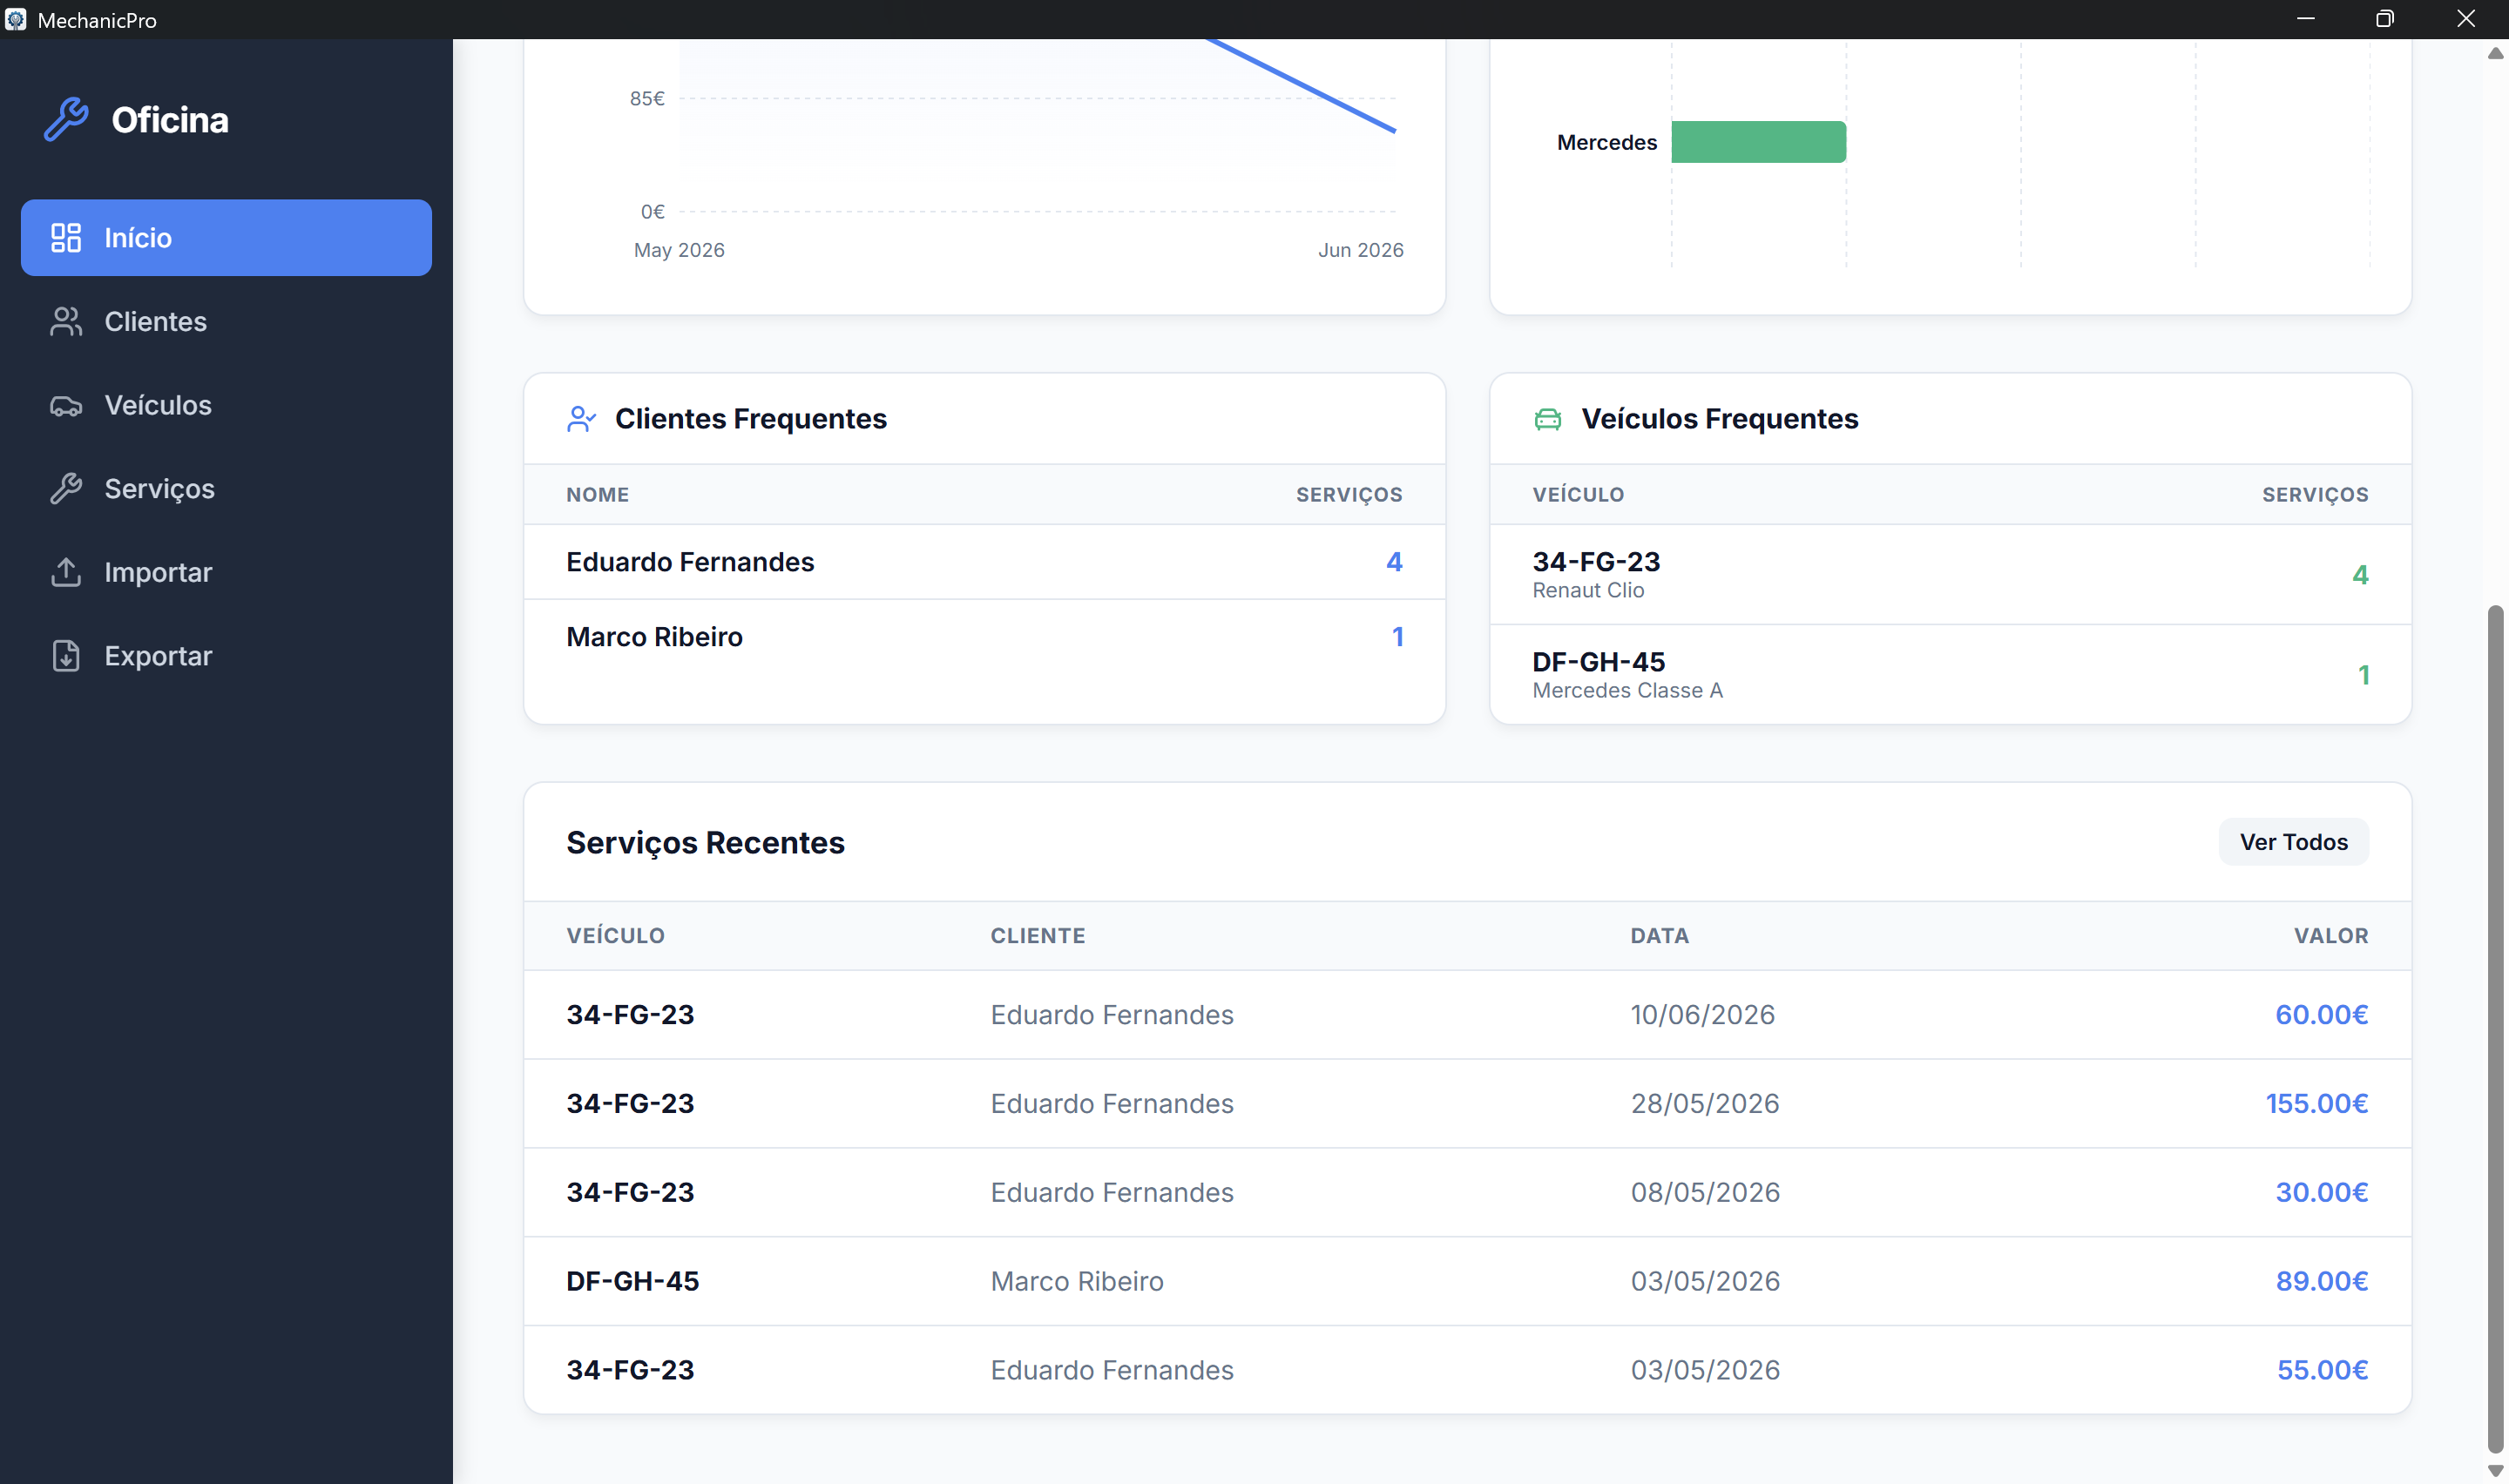
\includegraphics[width=0.9\textwidth]{figures/dashboard.png}
		\caption{Dashboard Page}
		\label{fig:dashboard_page}
	\end{figure}
	
	% =============================================================
	%  CHAPTER 4 --- CLIENTS
	% =============================================================
	\chapter{Managing Clients}
	
	\section{Viewing the Client List}
	To view your clients, click on \ui{Clients} in the sidebar. This opens a table displaying all registered vehicle owners. You can use the search bar at the top to quickly find a client by their name or phone number (see Figure~\ref{fig:clientes_listing}).
	
    \begin{figure}[H]
		\centering
		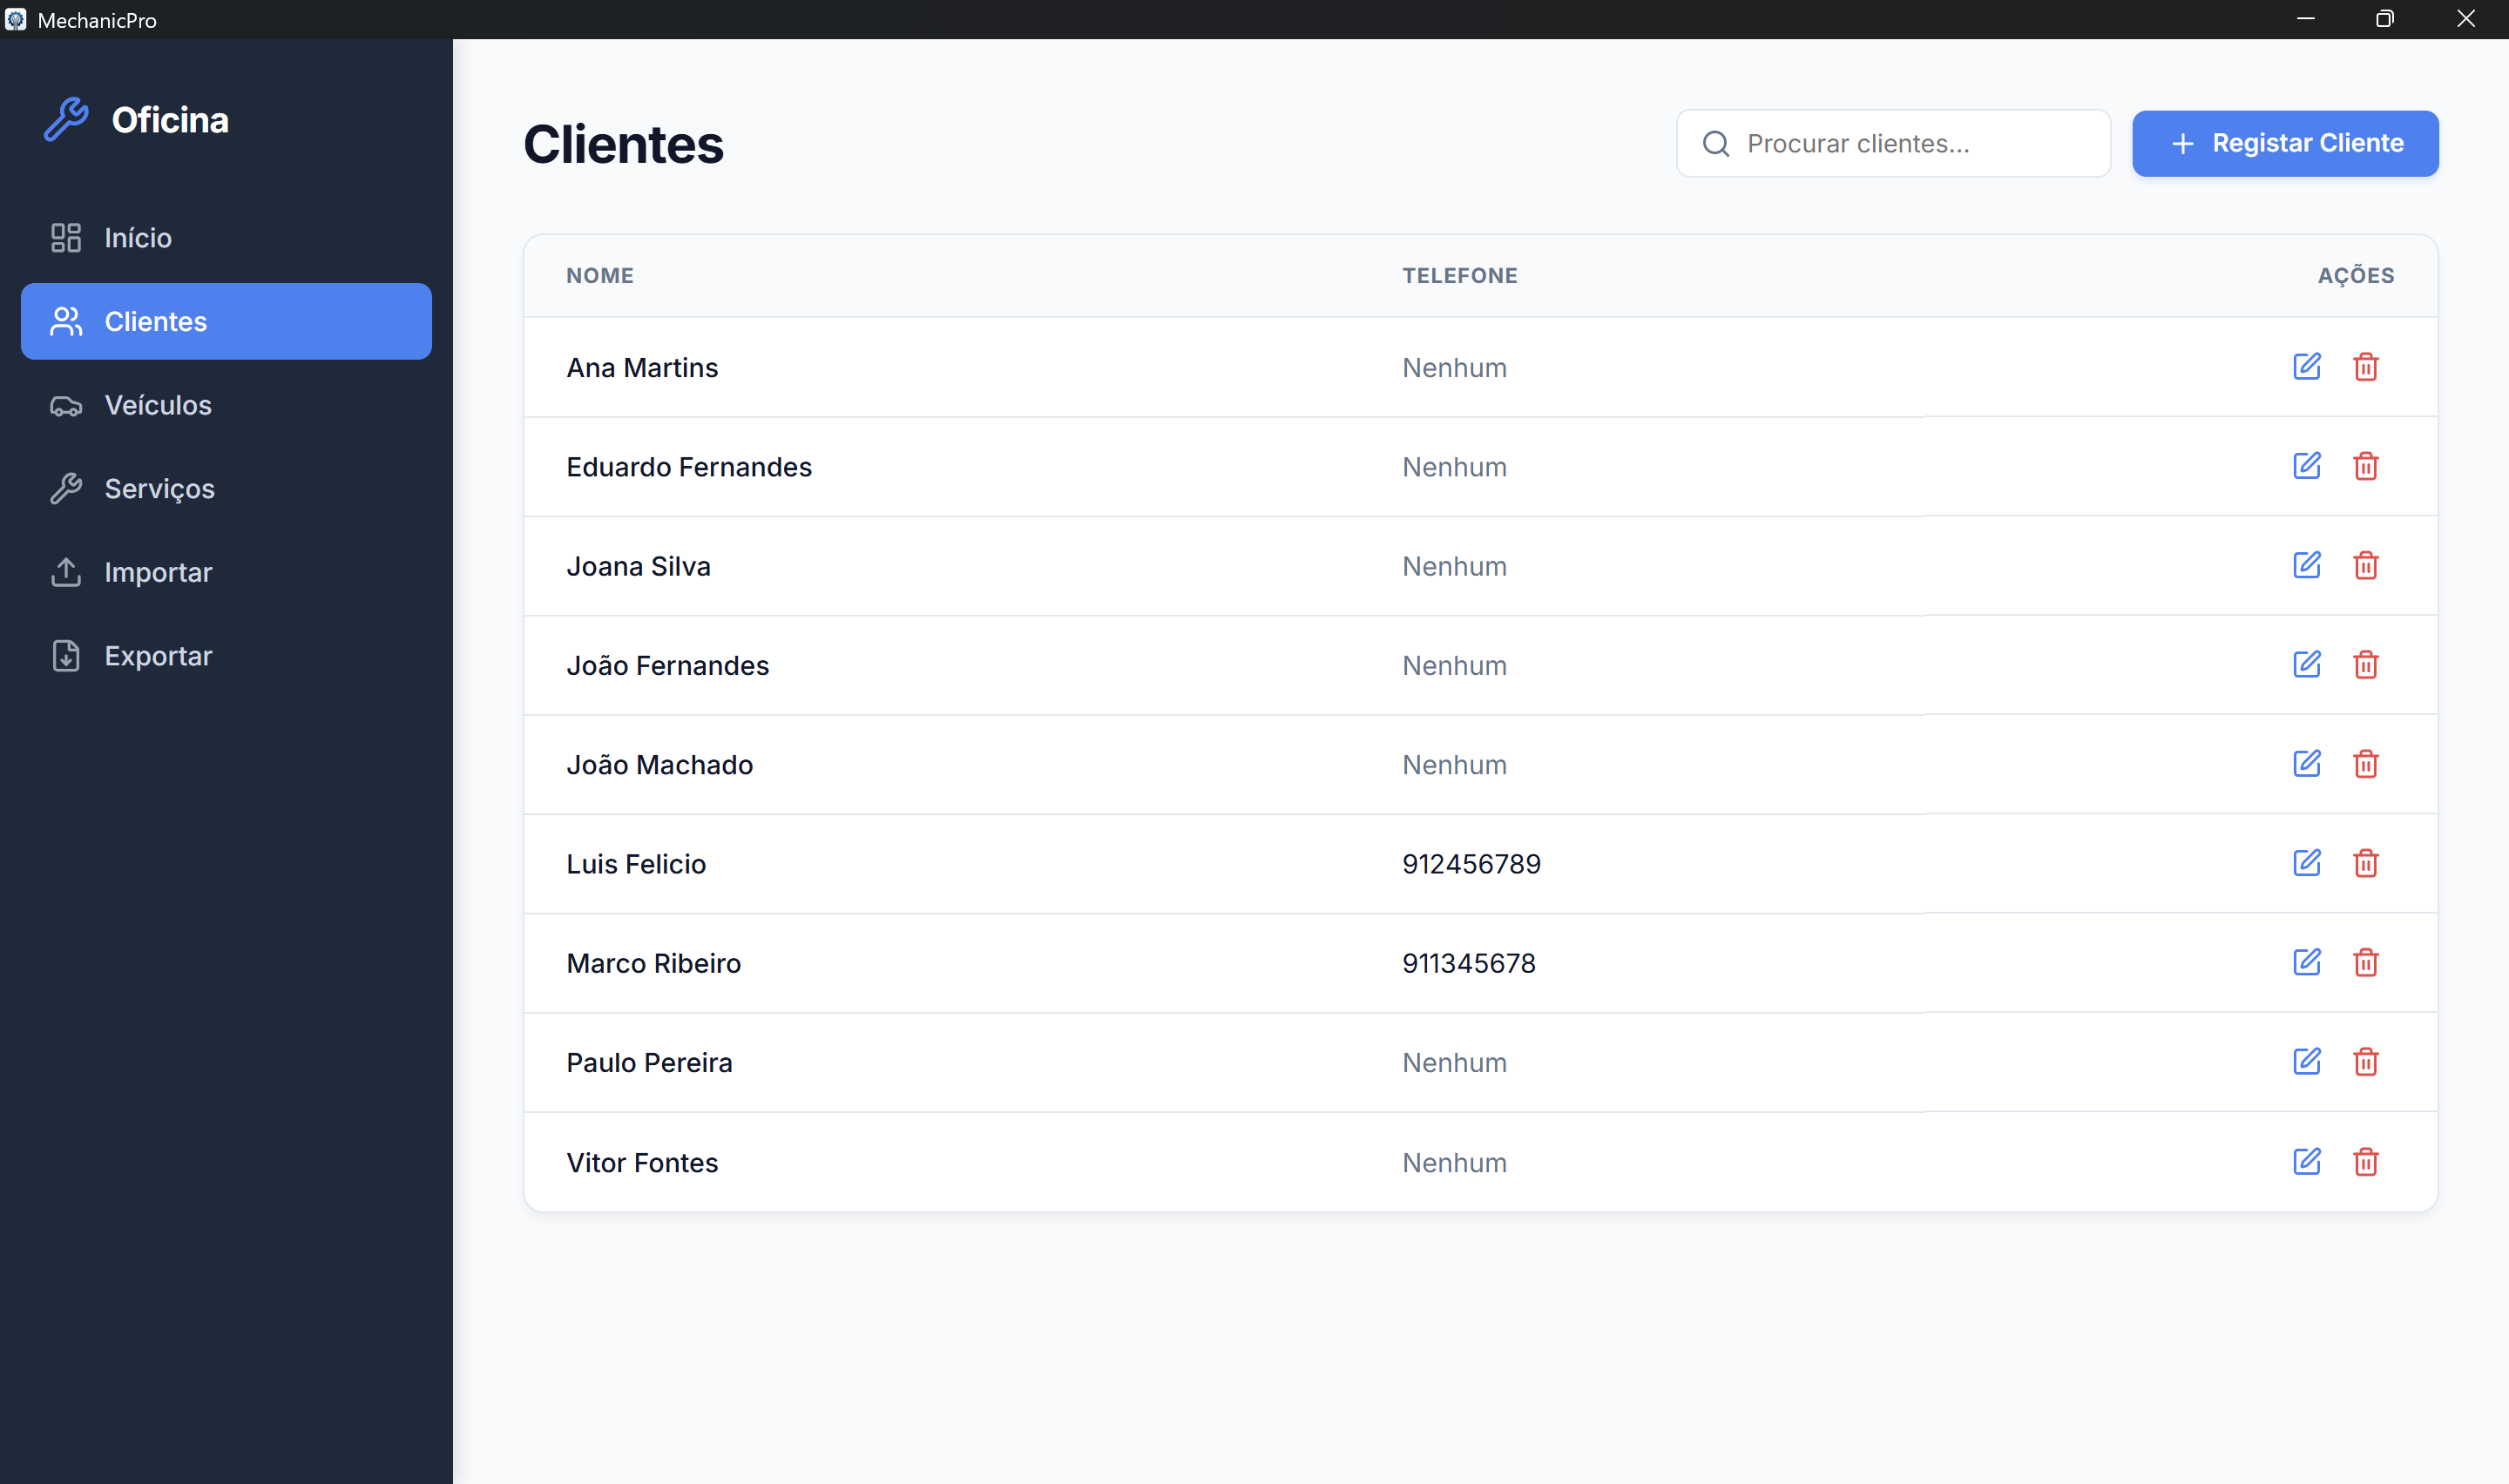
\includegraphics[width=0.9\textwidth]{figures/clientes.png}
		\caption{Clients listing page}
		\label{fig:clientes_listing}
	\end{figure}
    
	\section{Adding a Client}
	
	\begin{steps}
		\item Navigate to the \ui{Clients} section.
		\item Click the \ui{New Client} button.
		\item In the modal that appears, fill in the fields:
		\begin{itemize}
			\item \ui{Name}: full name of the client (required). Note that you cannot have two active clients with the exact same name.
			\item \ui{Phone}: contact phone number (optional).
		\end{itemize}
		\item Click \ui{Save}. The list will automatically update to show the new client.
	\end{steps}
	
	\section{Editing or Deleting a Client}
	
	\begin{steps}
		\item Locate the client in the list using the search bar.
		\item Click the \ui{Edit} icon next to their name.
		\item Update their Name or Phone number as needed, and click \ui{Save}.
		\item To remove the client, click the \ui{Delete} button.
	\end{steps}
	
	\dangerbox{Deleting a client does not permanently erase them from the database, but it hides them from all active lists. You can re-use their name for a new client later.}
	
	You can also view the history of a client, as shown in Figure~\ref{fig:client_history}.
	
    \begin{figure}[H]
		\centering
		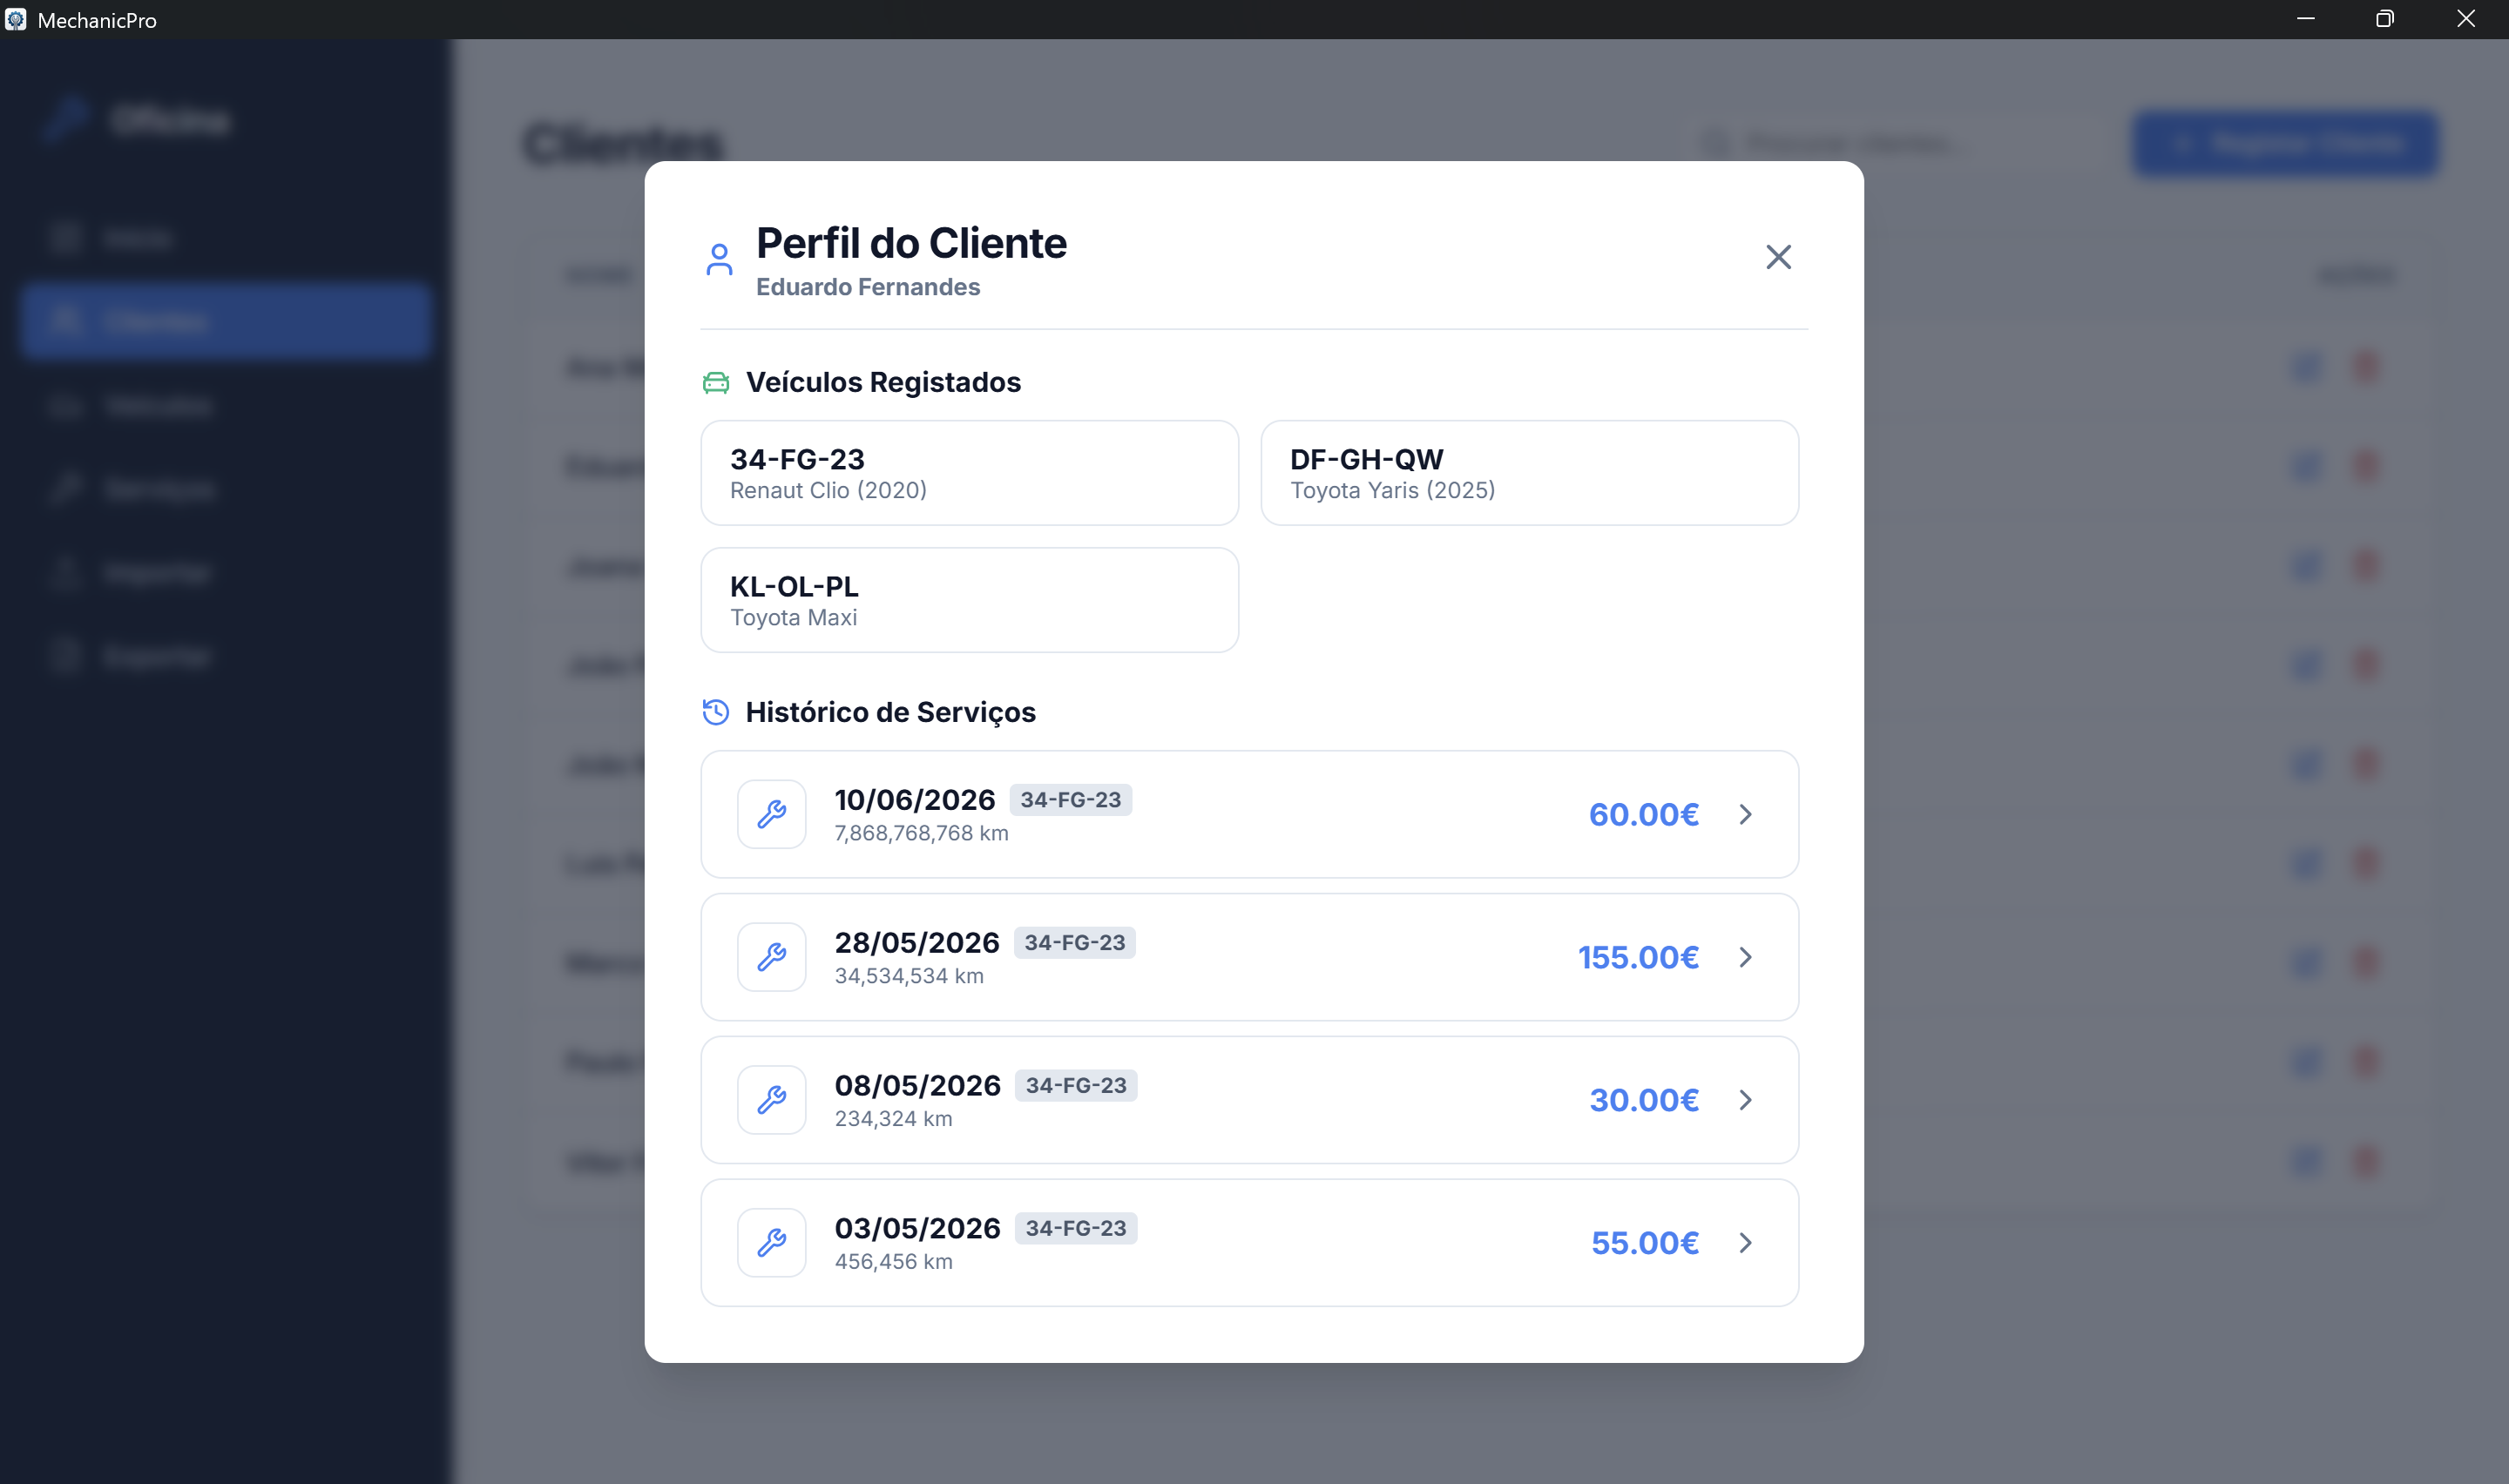
\includegraphics[width=0.9\textwidth]{figures/historico_cliente.png}
		\caption{Client history overlay}
		\label{fig:client_history}
	\end{figure}
    
	% =============================================================
	%  CHAPTER 5 --- VEHICLES
	% =============================================================
	\chapter{Managing Vehicles}
	
	\section{Viewing the Vehicle List}
	Click \ui{Vehicles} in the sidebar to access the complete list of cars registered in the system. Each vehicle is inextricably linked to a specific client. You can use the search bar to locate a vehicle by its Licence Plate or Make (see Figure~\ref{fig:vehicles_page}).
	
	\begin{figure}[H]
		\centering
		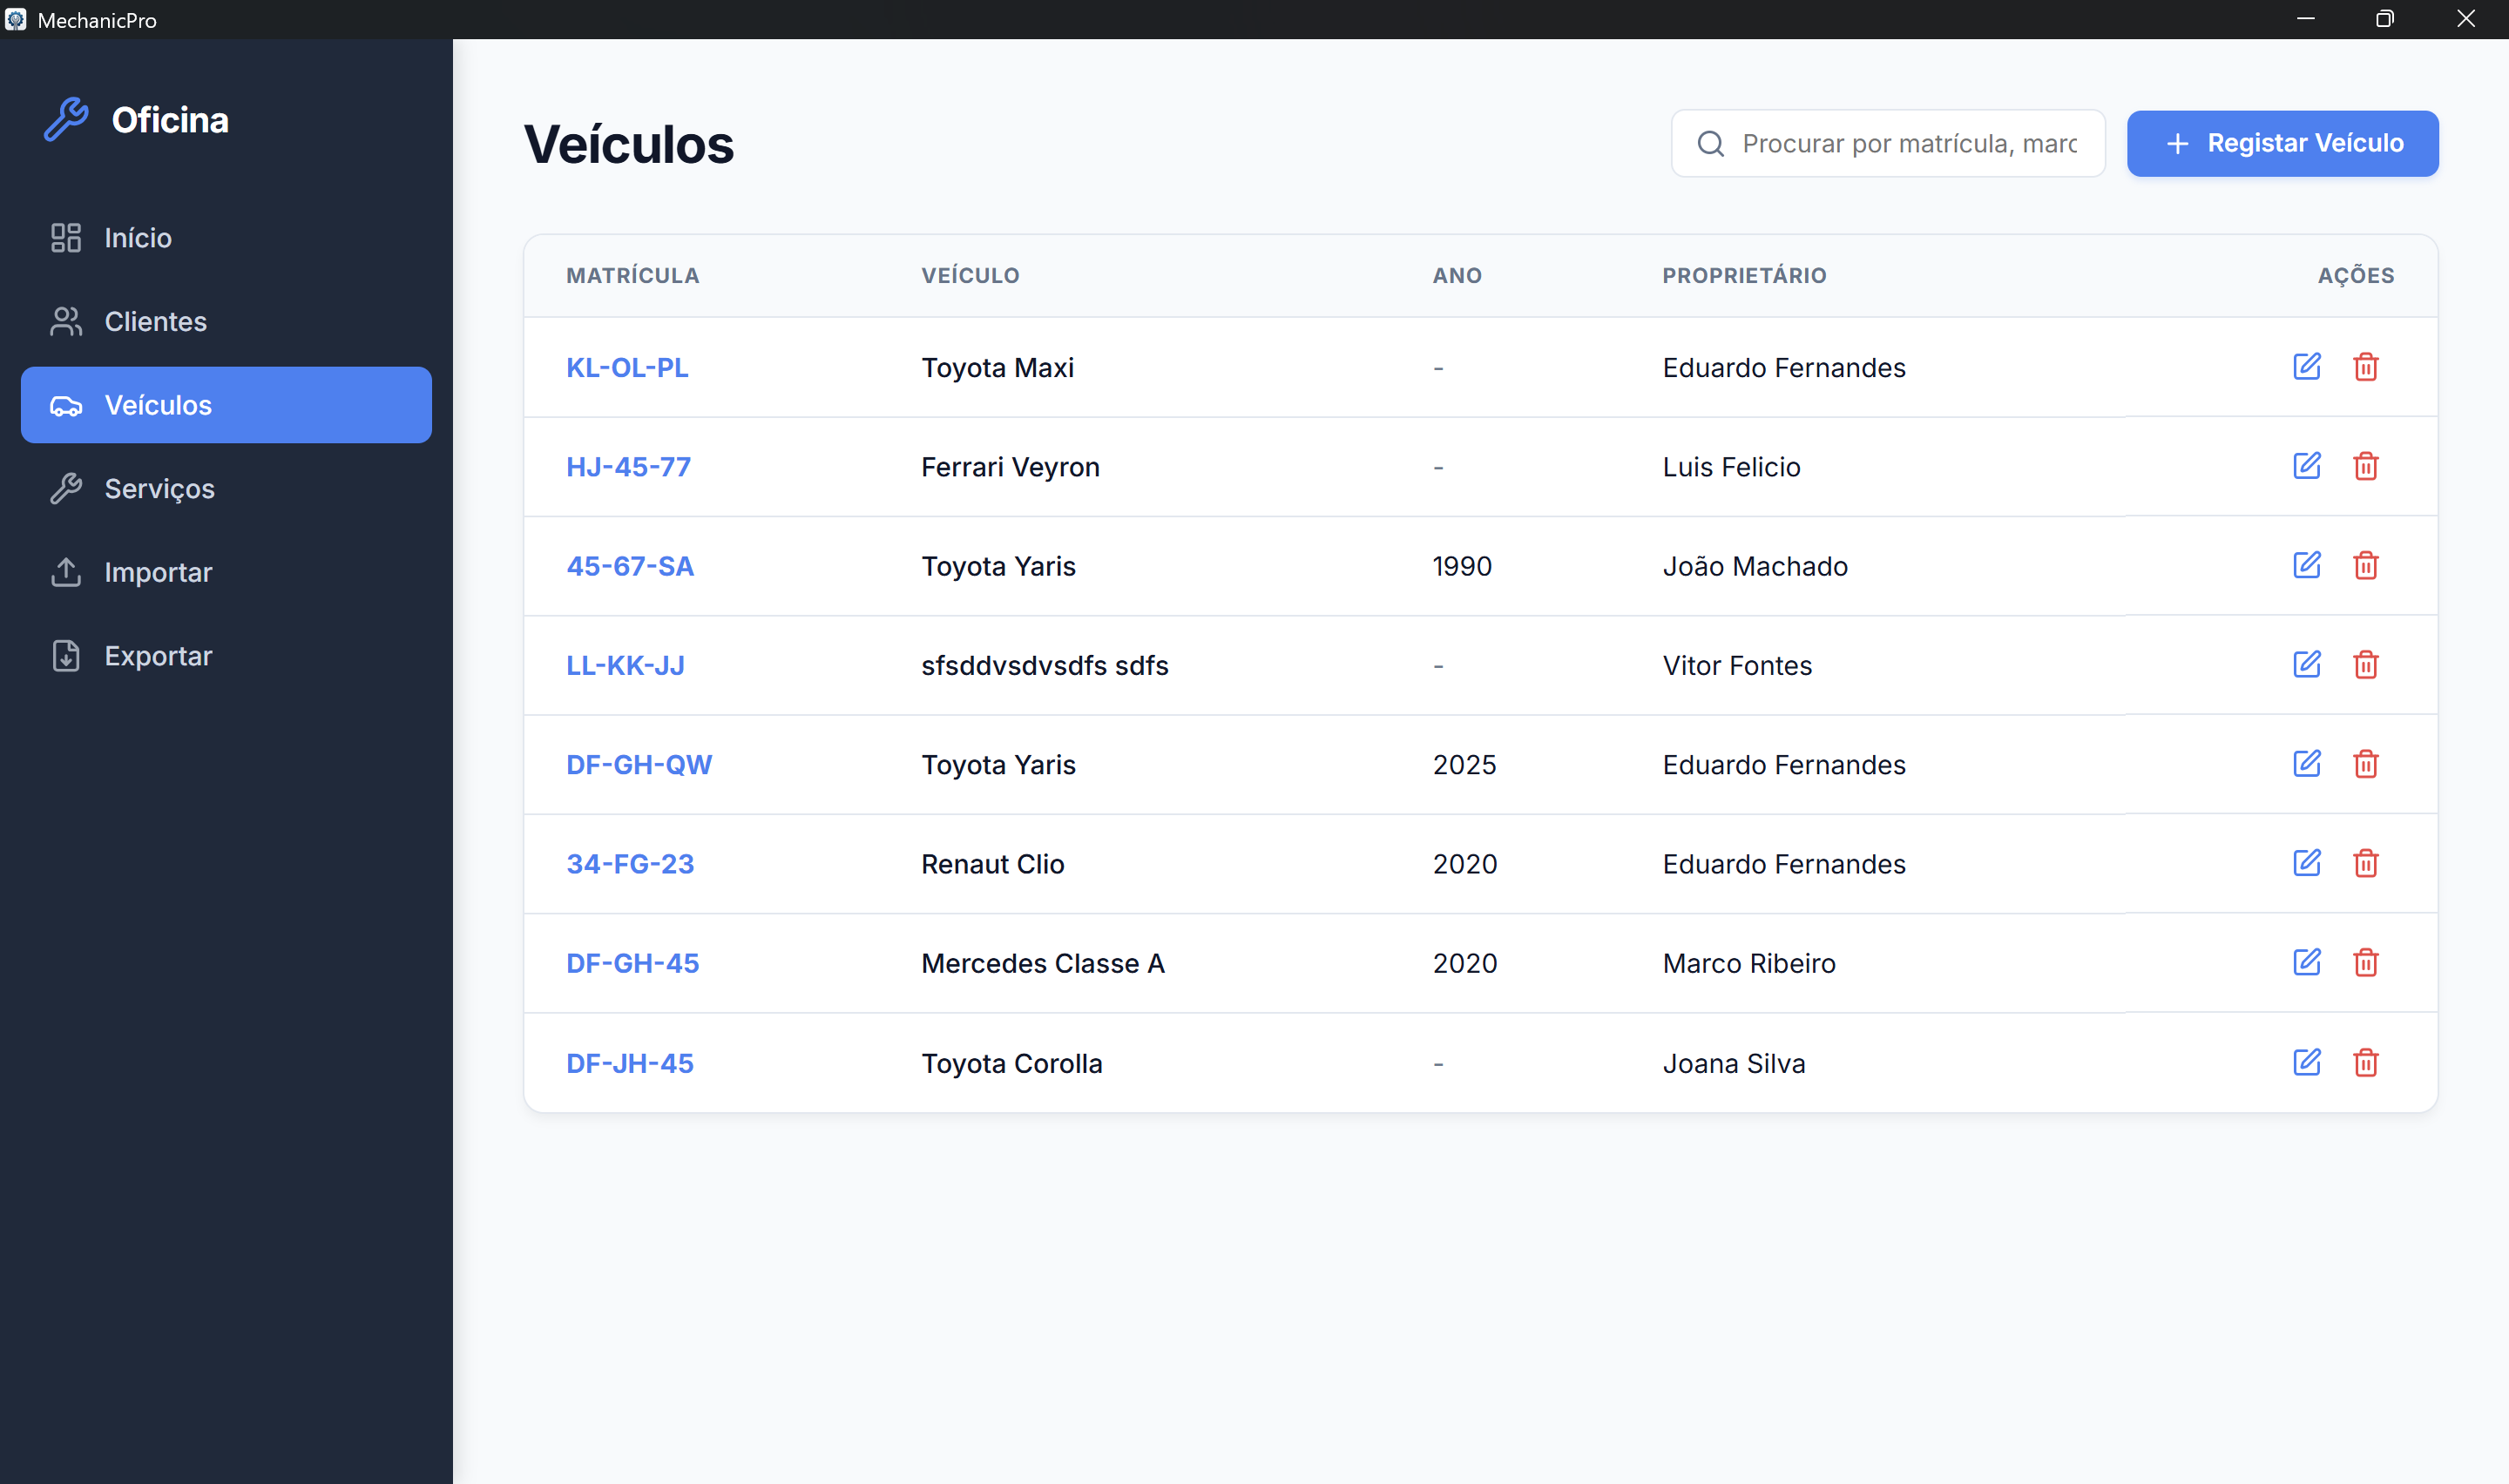
\includegraphics[width=0.9\textwidth]{figures/veiculos.png}
		\caption{Vehicles listing page}
		\label{fig:vehicles_page}
	\end{figure}
    
	\section{Adding a Vehicle}
	
	\begin{steps}
		\item Navigate to the \ui{Vehicles} section.
		\item Click \ui{New Vehicle}.
		\item Fill in the required fields:
		\begin{itemize}
			\item \ui{Licence Plate}: unique identifier for the vehicle (required).
			\item \ui{Make}: manufacturer name.
			\item \ui{Model}: vehicle model.
			\item \ui{Year}: year of manufacture.
			\item \ui{Owner}: select the associated client.
		\end{itemize}
		\item Click \ui{Save}.
	\end{steps}
	
	\section{Editing or Deleting a Vehicle}
	
	\begin{steps}
		\item Locate the vehicle in the list using the search bar.
		\item Click the \ui{Edit} icon next to its plate.
		\item Update the fields as needed, and click \ui{Save}.
		\item To remove the vehicle, click the \ui{Delete} button.
	\end{steps}
	
	\dangerbox{Deleting a vehicle hides it from active lists, but its historical service records are preserved for auditing purposes.}
	
	You can review the historical records for any vehicle (see Figure~\ref{fig:vehicles_history}).

    \begin{figure}[H]
		\centering
		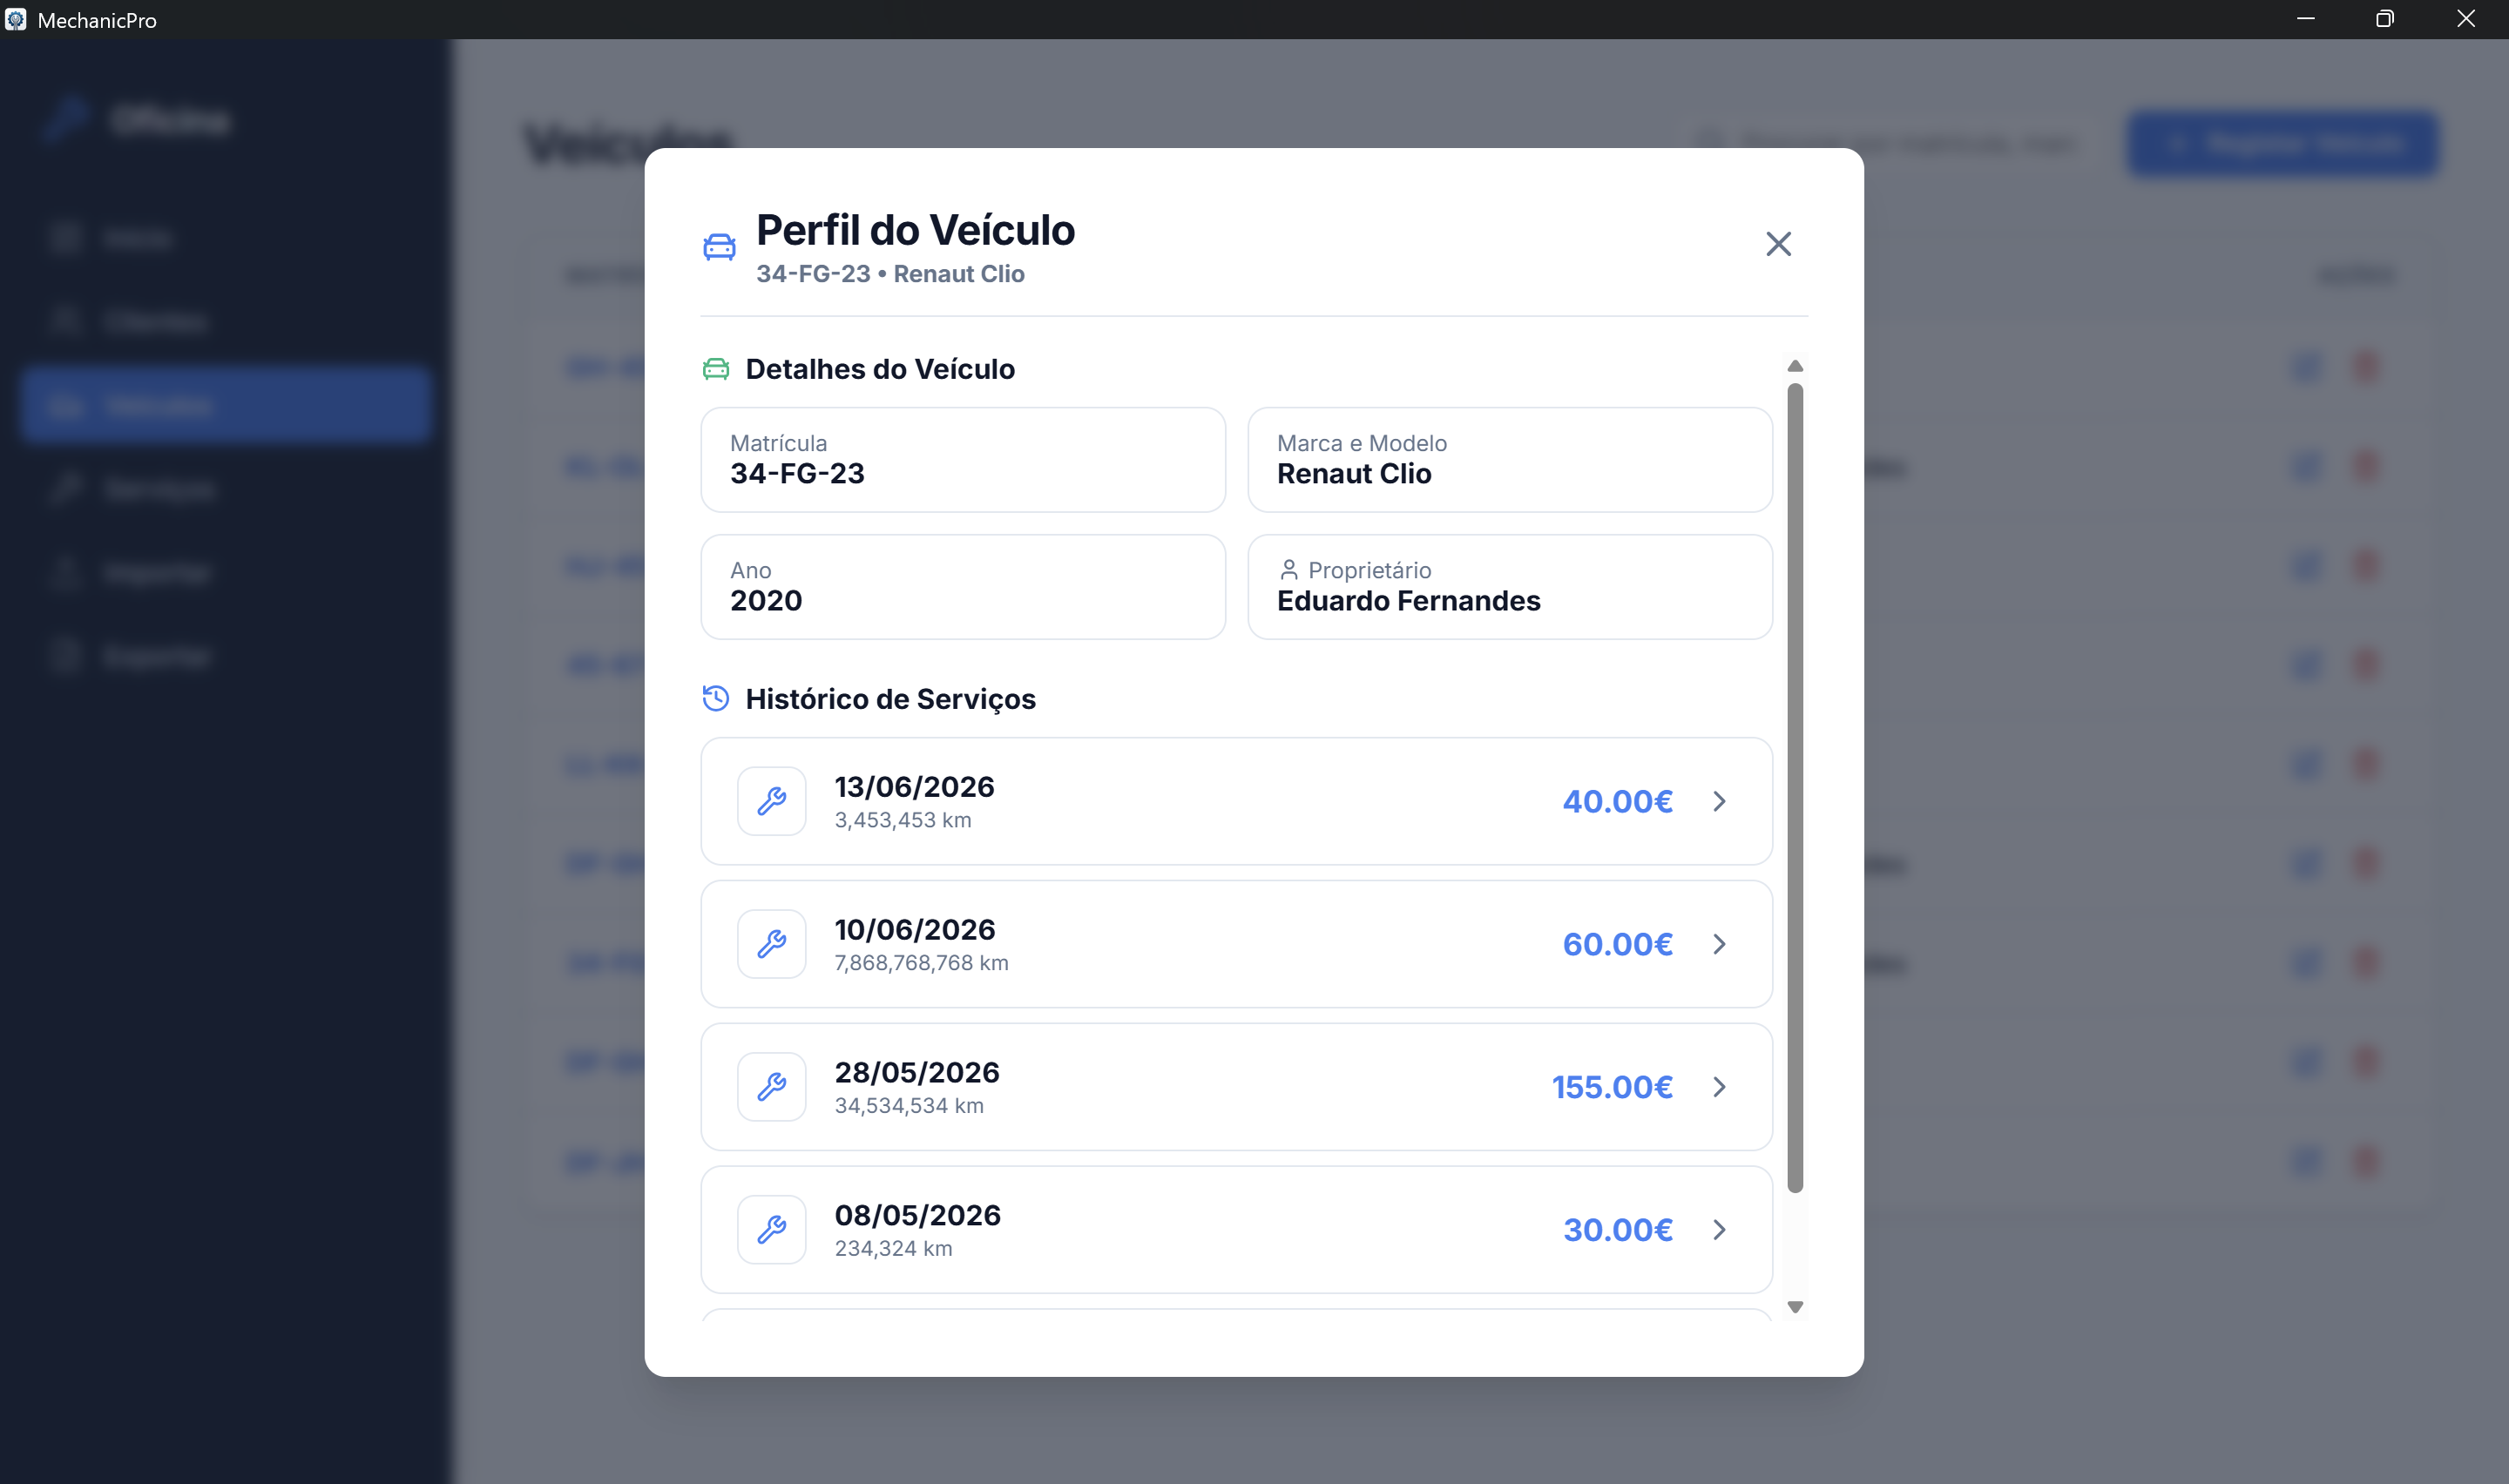
\includegraphics[width=0.9\textwidth]{figures/historico_veiculo.png}
		\caption{Vehicle history overlay}
		\label{fig:vehicles_history}
	\end{figure}
    
	% =============================================================
	%  CHAPTER 6 --- SERVICE ORDERS
	% =============================================================
	\chapter{Service Orders}
	
	\section{Overview}
	A Service Order is the core document in MechanicPro. It records a specific job performed on a vehicle. It includes the vehicle's mileage, itemized operations (parts or tasks), total labor hours, your hourly rate, and the final calculated price.
	
	\section{Creating a Service Order}
	
	\begin{steps}
		\item Navigate to \ui{Service Orders}.
		\item Click \ui{New Order}.
		\item Select the \ui{Client} and their associated \ui{Vehicle}.
		\item Record the current \ui{Mileage} of the vehicle.
		\item Add any general notes in the \ui{Observations} field.
		\item Add individual \ui{Operations} (such as parts or specific tasks), giving each a description and a price.
		\item Enter the total labor \ui{Hours} and your \ui{Hourly Rate}. The total price will calculate automatically based on the operations and labor.
		\item Click \ui{Save}.
	\end{steps}
	
	Figure~\ref{fig:create_service_order} illustrates the creation of a new service order.
	
	\begin{figure}[H]
		\centering
		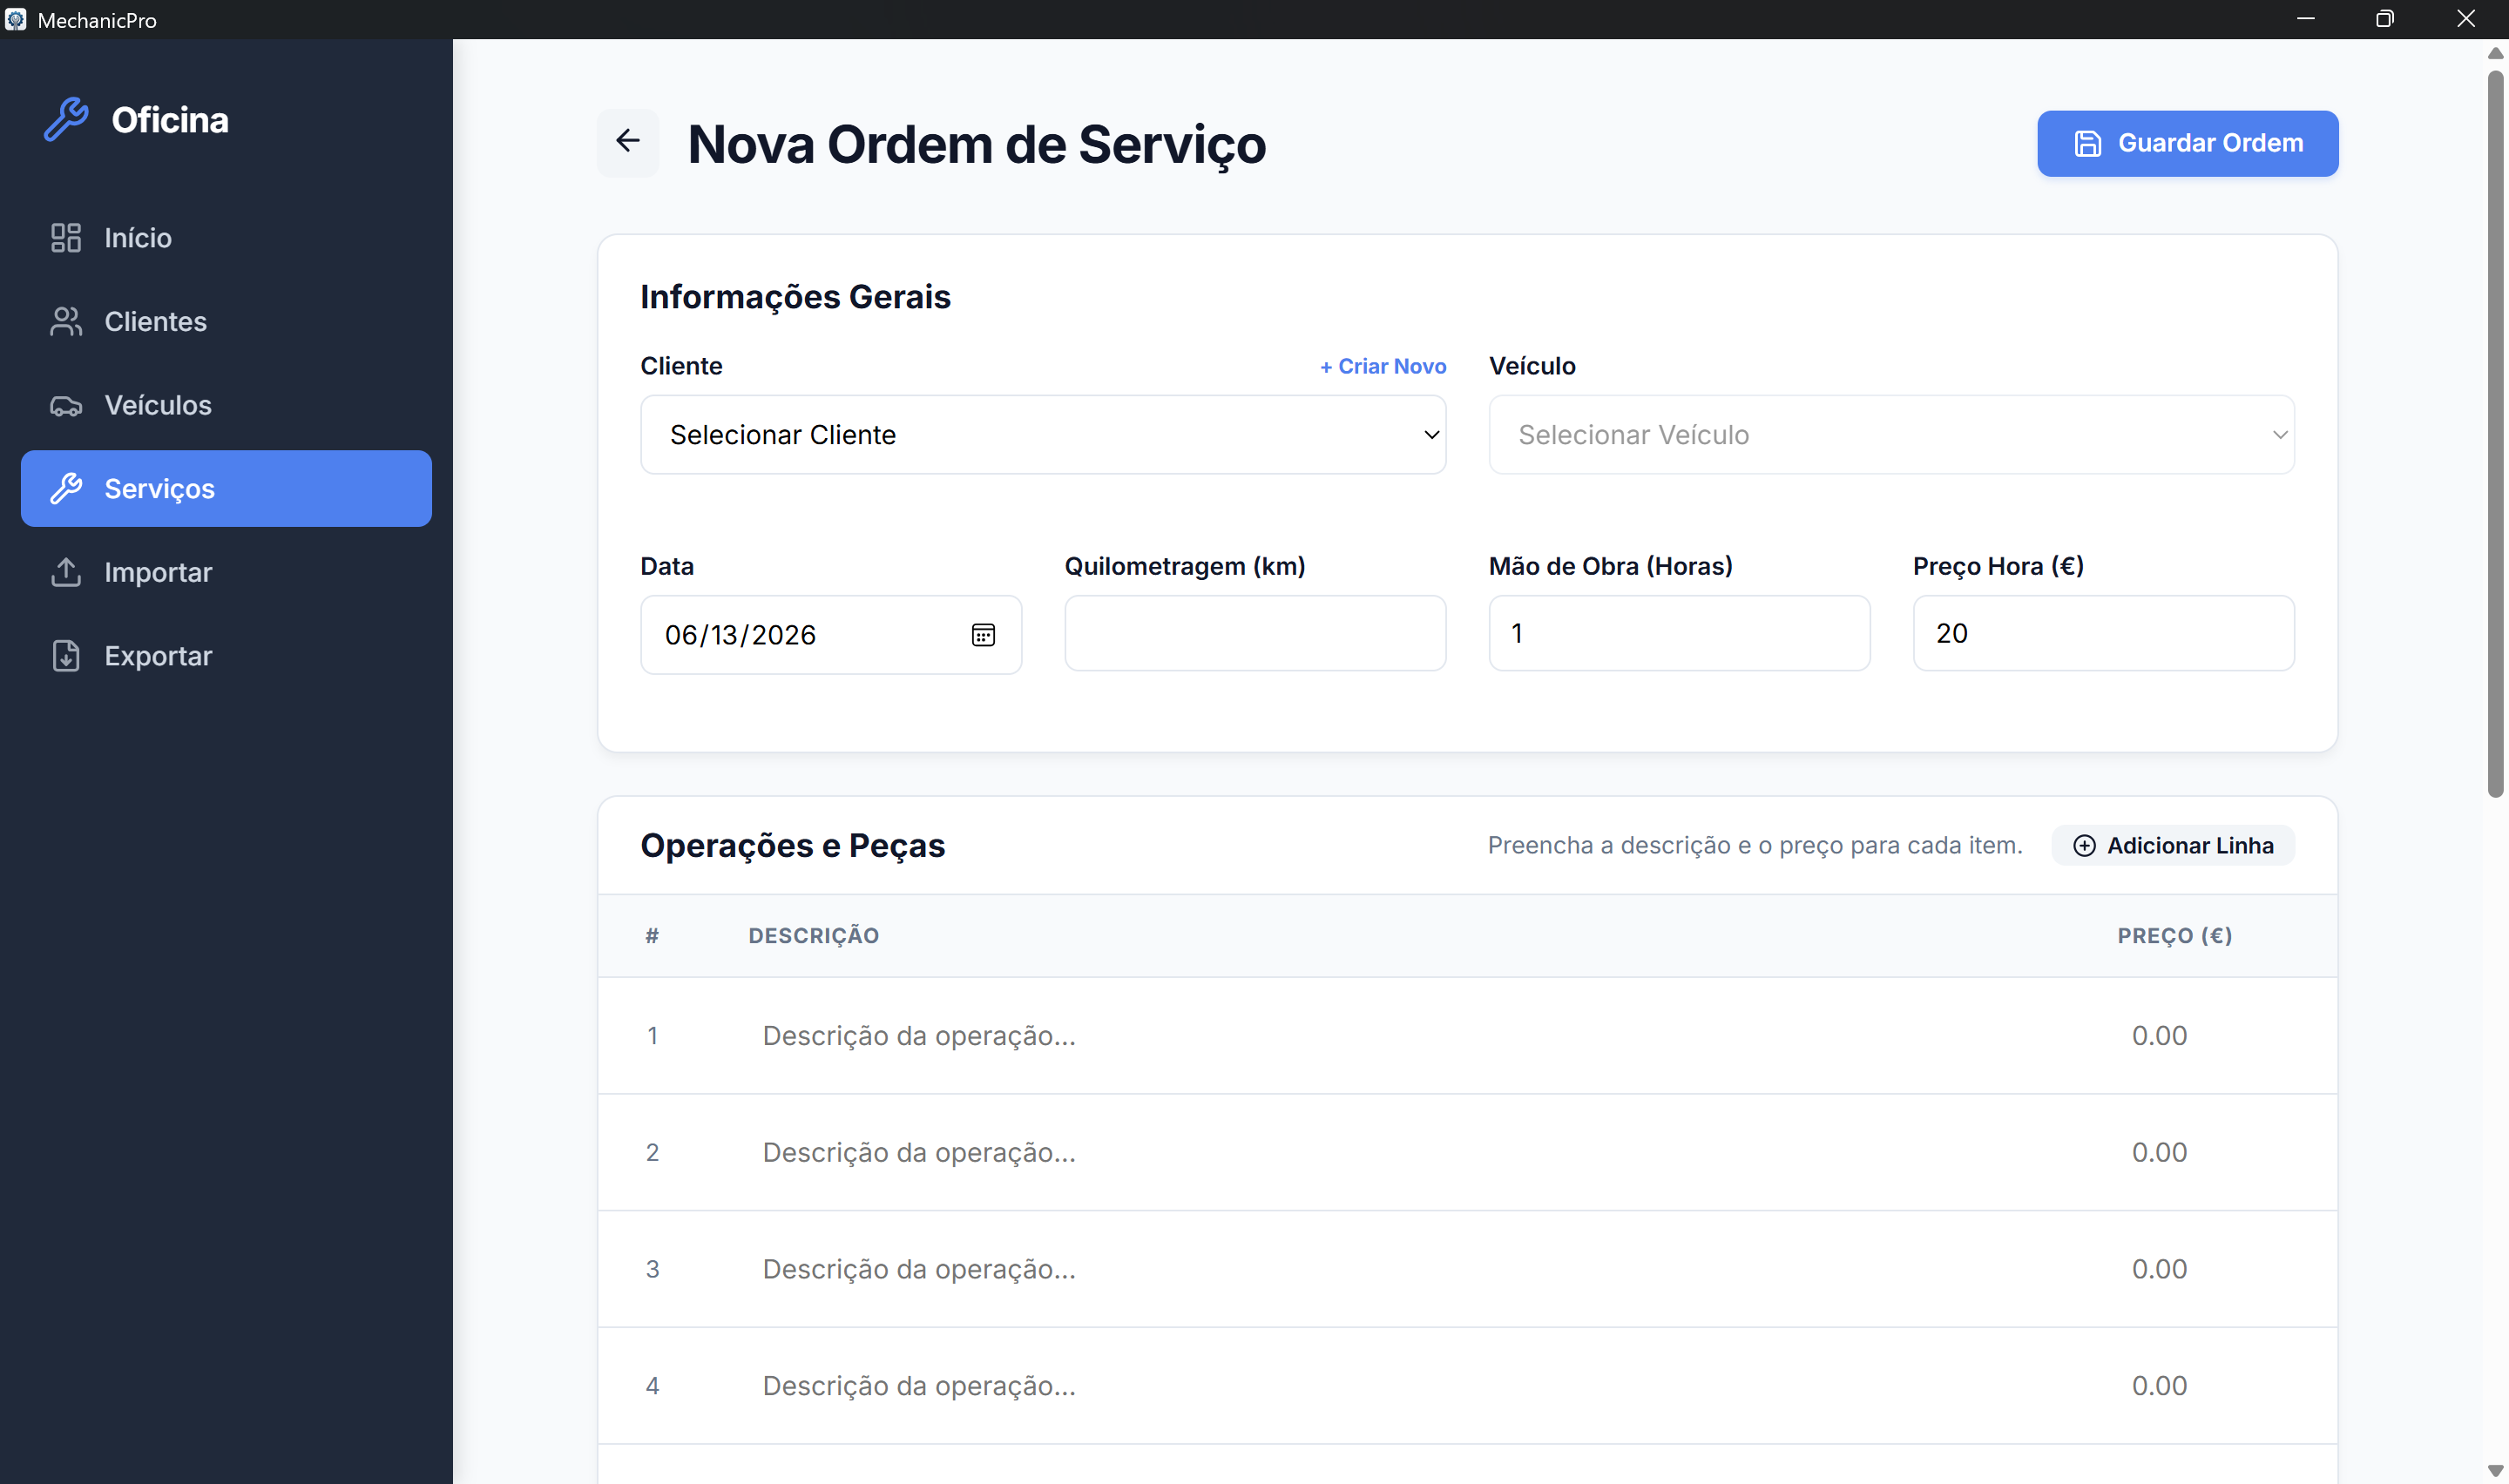
\includegraphics[width=0.9\textwidth]{figures/criar_servico.png}
		\caption{Creating a new Service Order}
		\label{fig:create_service_order}
	\end{figure}
	
	\section{Sorting Service Orders}
	By default, service orders are listed chronologically. You can click the column headers in the Service Orders table to change the sorting (for example, sorting by Date in descending order to see the newest jobs first, or by Total Price to see the most expensive jobs).
	
	\section{Viewing Service History}
	To see a history of all past service orders, you can view the main Service Orders list. Alternatively, viewing a specific Vehicle's profile will show a timeline of all service orders associated with that specific car (see Figure~\ref{fig:service_history}).
	
	\begin{figure}[H]
		\centering
		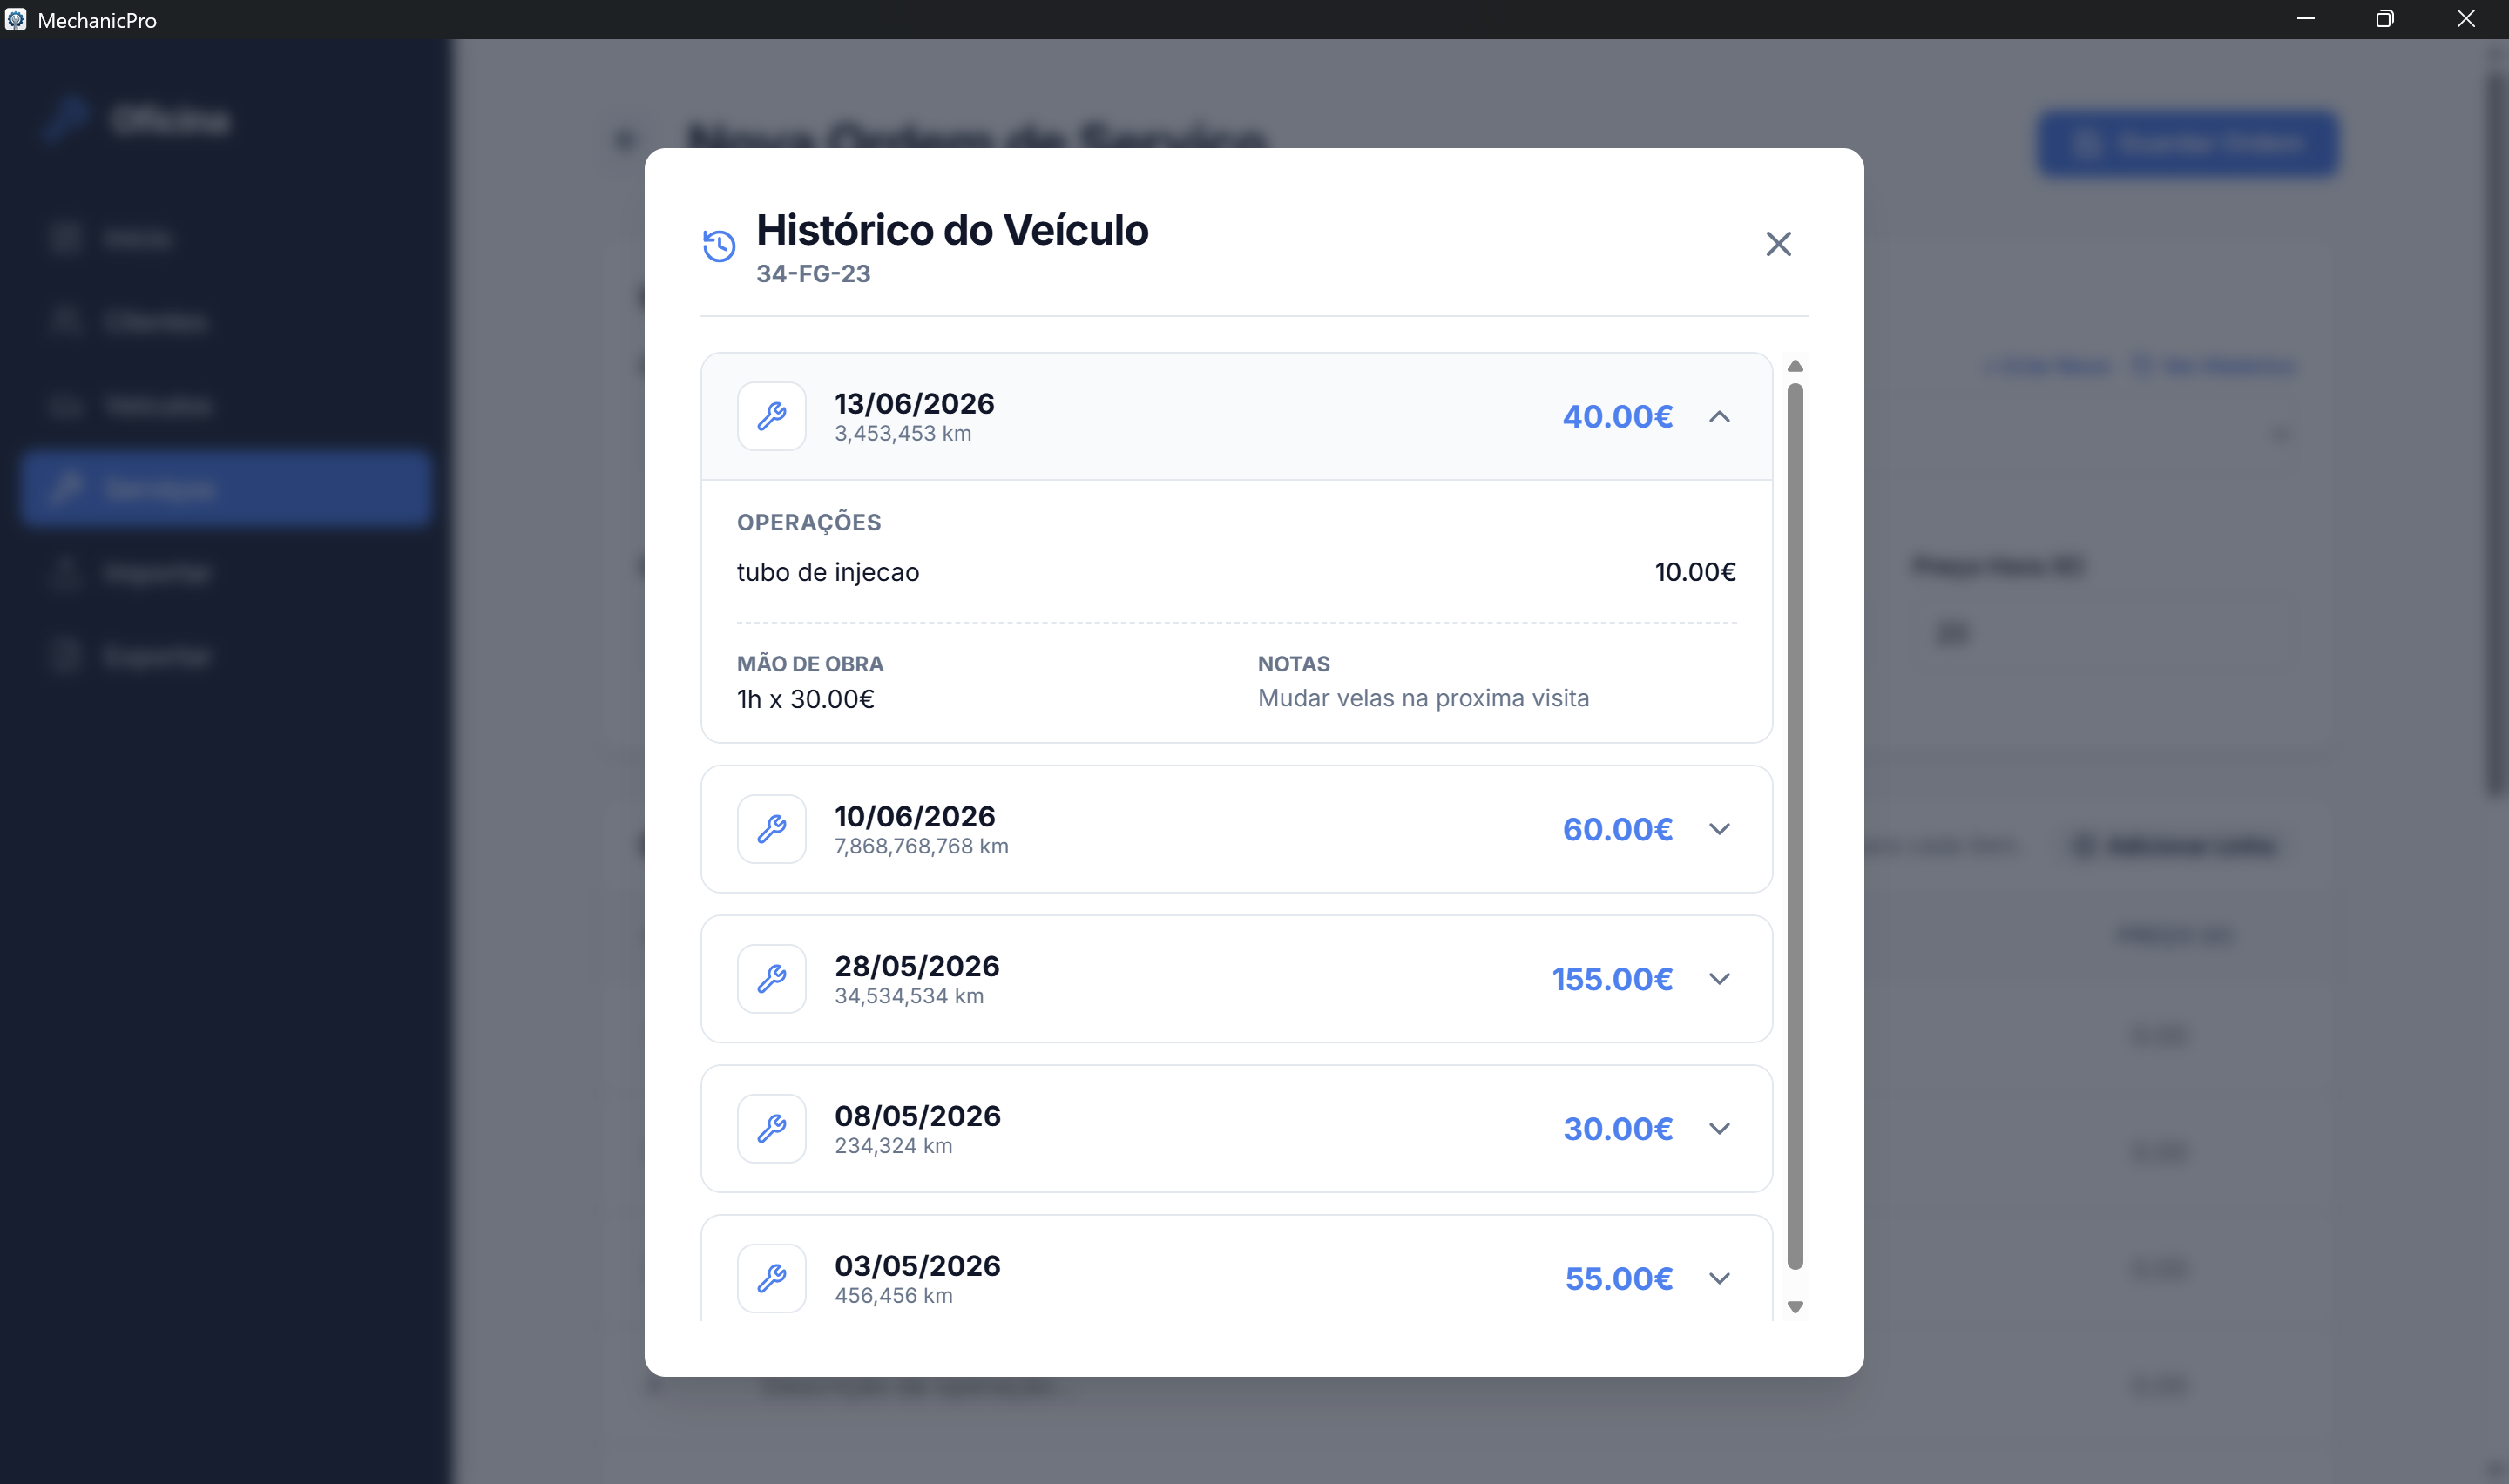
\includegraphics[width=0.9\textwidth]{figures/ver_historico.png}
		\caption{Service History View}
		\label{fig:service_history}
	\end{figure}
	
	\section{Downloading Service Details}
	Once a service order is finalized, you can generate a professional PDF invoice to print or email to your customer. Simply open the service order details and click the \ui{Download PDF} button. See Chapter 8 for more information on PDF generation.
	
	% =============================================================
	%  CHAPTER 7 --- DASHBOARD
	% =============================================================
	\chapter{Dashboard}
	
	\section{Overview}
	The Dashboard provides an immediate snapshot of your shop's health and workload. It is designed to be a quick reference point rather than a detailed management screen (see Figure~\ref{fig:dashboard_overview}).
	
	\begin{figure}[H]
		\centering
		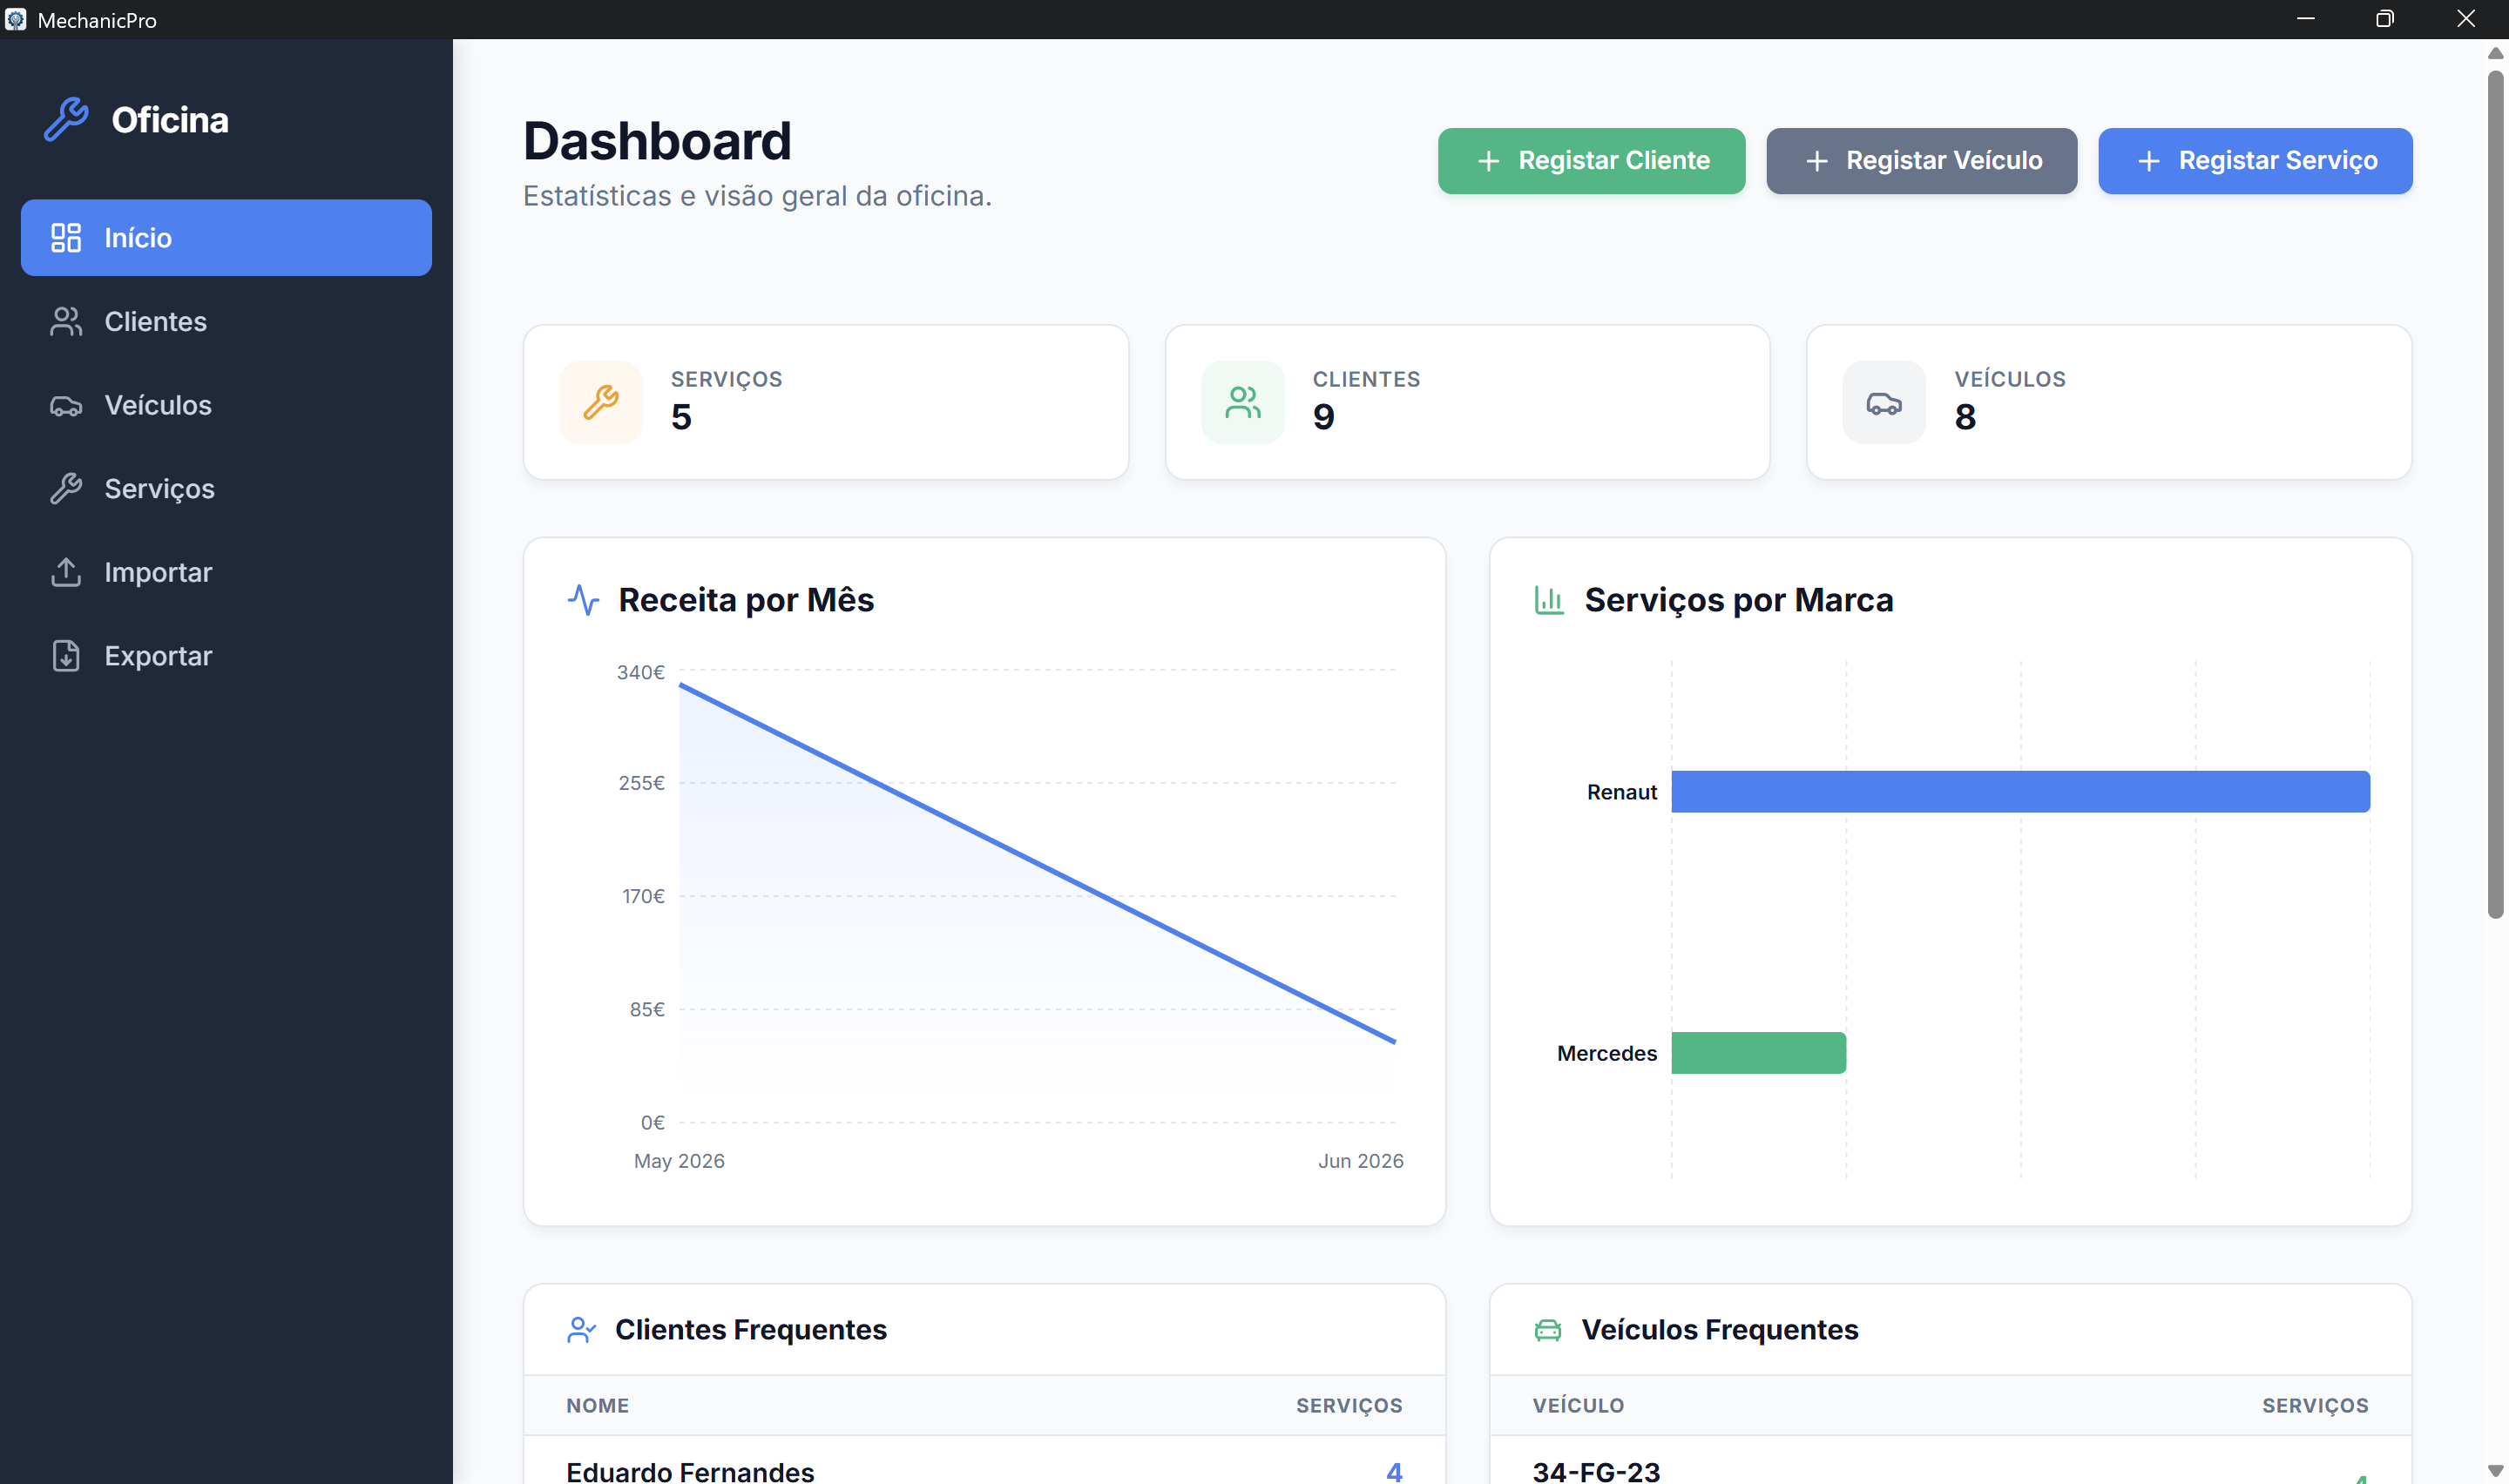
\includegraphics[width=0.9\textwidth]{figures/sidebar_main_content.png}
		\caption{Dashboard Overview}
		\label{fig:dashboard_overview}
	\end{figure}
	
	\section{Statistics and Top Lists}
	At the top of the dashboard, you will see key performance indicators:
	\begin{itemize}
		\item \ui{Serviços} (Total Services): The total number of service orders recorded.
		\item \ui{Clientes} (Total Clients): The number of active clients.
		\item \ui{Veículos} (Total Vehicles): The number of active vehicles.
	\end{itemize}
	
	Below the key metrics, you will find quick-reference lists for your \ui{Frequent Clients} and \ui{Frequent Vehicles}, ranking those with the most recorded services, as well as a list of \ui{Recent Services} for quick access.
	
	\section{Charts}
	The dashboard also includes interactive charts to visualize your shop's trends:
	\begin{itemize}
		\item \ui{Revenue by Month}: An area chart showing the total value of services performed each month.
		\item \ui{Services by Brand}: A bar chart showing the breakdown of vehicles serviced by their manufacturer.
	\end{itemize}
	You can hover over the data points in these charts to see exact numbers.
	
	% =============================================================
	%  CHAPTER 8 --- DATA MANAGEMENT
	% =============================================================
	\chapter{Data Management}
	
	\section{Exporting Data to CSV}
	MechanicPro allows you to export your data (Clients, Vehicles, and Service Orders) at any time to standard CSV files, which can be opened in Excel or Google Sheets.
	
	\begin{steps}
		\item Navigate to the \ui{Import / Export} section in the sidebar.
		\item Under the Export tab, select the type of data you wish to export.
		\item Click \ui{Export CSV}.
		\item Choose a location on your computer to save the file.
	\end{steps}
	
	\section{Importing Data from CSV}
	You can bulk-import clients and vehicles from existing spreadsheets to save time during initial setup.
	
	\warnbox{Importing a CSV file will add records to the existing data.
		It does not replace or delete current records.}
	
	\subsection{Required CSV Format}
	
	The import file must use UTF-8 encoding. The columns must exactly match the system's requirements:
	
	\subsubsection*{Clients CSV}
	
	The expected structure for the clients CSV file is detailed in Table~\ref{tab:csv_clients}.

	\begin{table}[H]
		\centering
		\caption{Required CSV Format: Clients}
		\label{tab:csv_clients}
		\begin{tabularx}{\textwidth}{l l X}
			\toprule
			\textbf{Column} & \textbf{Required} & \textbf{Notes} \\
			\midrule
			name   & Yes & Full name of the client \\
			phone  & No  & Contact number \\
			\bottomrule
		\end{tabularx}
	\end{table}
	
	\vspace{10pt}
	\subsubsection*{Vehicles CSV}
	
	The expected structure for the vehicles CSV file is detailed in Table~\ref{tab:csv_vehicles}.

	\begin{table}[H]
		\centering
		\caption{Required CSV Format: Vehicles}
		\label{tab:csv_vehicles}
		\begin{tabularx}{\textwidth}{l l X}
			\toprule
			\textbf{Column} & \textbf{Required} & \textbf{Notes} \\
			\midrule
			plate  & Yes & Unique Licence Plate \\
			brand  & Yes & Manufacturer (Make) \\
			model  & Yes & Vehicle model \\
			year   & No  & Manufacturing year \\
			\bottomrule
		\end{tabularx}
	\end{table}
	
	\begin{steps}
		\item Navigate to the \ui{Import / Export} section.
		\item Select the type of data you are importing.
		\item Click \ui{Choose File} and select your CSV file.
		\item Review the preview to ensure the columns align correctly.
		\item Click \ui{Import}.
	\end{steps}
	
	\dangerbox{Records created by import cannot be automatically undone.
		Make an export backup before importing new data.}
	
	\section{Generating PDF Documents}
	MechanicPro includes a built-in PDF generator for creating professional invoices and service summaries.
	
	\begin{steps}
		\item Open a finalized service order from the \ui{Service Orders} list.
		\item Review the total cost, mileage, and itemized lists to ensure accuracy.
		\item Click the \ui{Download PDF} button.
		\item The PDF will be saved to your computer, ready to be printed or emailed to the client.
	\end{steps}
	
	% =============================================================
	%  CHAPTER 9 --- TROUBLESHOOTING
	% =============================================================
	\chapter{Troubleshooting}
	
	\section{Common Issues}
	
	Table~\ref{tab:common_issues} lists some common issues and their solutions.

	\begin{table}[H]
		\centering
		\caption{Common Troubleshooting Issues}
		\label{tab:common_issues}
		\begin{tabularx}{\textwidth}{l X}
			\toprule
			\textbf{Problem} & \textbf{Solution} \\
			\midrule
			Application does not open
			& Check that WebView2 is installed (Windows only).
			Try reinstalling the application. \\
			\addlinespace
			CSV import fails
			& Verify the file is UTF-8 encoded and that all required
			columns are present with the correct header names. \\
			\addlinespace
			Data appears missing after reinstall
			& The database is stored separately from the application.
			See Section~\ref{sec:dataLocation} for the file location. \\
			\addlinespace
			PDF does not download
			& Check that you have write permission to the chosen folder. \\
			\bottomrule
		\end{tabularx}
	\end{table}
	
	\section{Data File Location}
	\label{sec:dataLocation}
	If you need to manually back up your database file, or if you are moving MechanicPro to a new computer, you can find the SQLite database file at the following standard locations depending on your operating system:
	
	\begin{itemize}
		\item \textbf{Windows}: \texttt{\%APPDATA\%\textbackslash{}MechanicPro\textbackslash{}mechanicpro.db}
		\item \textbf{macOS}: \texttt{\textasciitilde{}/Library/Application Support/MechanicPro/mechanicpro.db}
		\item \textbf{Linux}: \texttt{\textasciitilde{}/.local/share/MechanicPro/mechanicpro.db}
	\end{itemize}
	
	\notebox{You can back up your data by simply copying this \texttt{mechanicpro.db} file to a safe location (such as a USB drive or cloud folder) while the application is closed.}
	
	% =============================================================
	%  APPENDICES
	% =============================================================
	\appendix
	
	\chapter{Glossary}
	
	Table~\ref{tab:glossary} defines key terms used throughout this manual.

	\begin{table}[H]
		\centering
		\caption{Glossary of Terms}
		\label{tab:glossary}
		\begin{tabularx}{\textwidth}{l X}
			\toprule
			\textbf{Term} & \textbf{Definition} \\
			\midrule
			Client        & A person or entity whose vehicle is serviced. \\
			Vehicle       & A car or other vehicle registered under a client. \\
			Service Order & A record of a service performed or requested. \\
			CSV           & Comma-Separated Values. A plain text file format
			for tabular data. \\
			PDF           & Portable Document Format. A fixed-layout document
			format used for service records. \\
			\bottomrule
		\end{tabularx}
	\end{table}
	
	\chapter{Keyboard Shortcuts}
	
	There are currently no custom global keyboard shortcuts. Standard operating system shortcuts for copying (\key{Ctrl+C}) and pasting (\key{Ctrl+V}) apply within all text fields.
	
\end{document}